\documentclass[12pt,a4paper]{report}

\usepackage{tabularx}

\usepackage[utf8]{inputenc} % pentru suport diacritice
\usepackage[english]{babel} % setări pentru engleza 
\renewcommand\familydefault{\sfdefault} % sans serif

\usepackage[margin=2.54cm]{geometry}	% dimensiuni pagină și margini
\usepackage{graphicx} % support the \includegraphics command and options
\usepackage{subcaption}

\usepackage{lmodern}
\usepackage{newunicodechar}
\newunicodechar{β}{\ensuremath{\beta}}

% formatting sections and subsections
\usepackage{textcase}
\usepackage[titletoc, title]{appendix}
\usepackage{titlesec}
\titleformat{\chapter}{\large\bfseries\MakeUppercase}{\thechapter}{2ex}{}[\vspace*{-1.5cm}]
\titleformat*{\section}{\large\bfseries}
\titleformat*{\subsection}{\large\bfseries}
\titleformat*{\subsubsection}{\large\bfseries}

\usepackage{chngcntr}
\counterwithout{figure}{chapter} % no chapter number in figure labels
\counterwithout{table}{chapter} % no chapter number in table labels
\counterwithout{equation}{chapter} % no chapter number in equation labels

\usepackage{booktabs} % for much better looking tables
\usepackage{url} % Useful for inserting web links nicely
\usepackage[bookmarks,unicode,hidelinks]{hyperref}

\usepackage{array} % for better arrays (eg matrices) in maths
\usepackage{paralist} % very flexible & customisable lists (eg. enumerate/itemize, etc.)
\usepackage{verbatim} % adds environment for commenting out blocks of text & for better verbatim
% deprecated
% \usepackage{subfig} % make it possible to include more than one captioned figure/table in a single float
\usepackage{enumitem}
\setlist{noitemsep}

%%% HEADERS & FOOTERS
\usepackage{fancyhdr}
\pagestyle{empty}
\renewcommand{\headrulewidth}{0pt}
\renewcommand{\footrulewidth}{0pt}
\lhead{}\chead{}\rhead{}
\lfoot{}\cfoot{\thepage}\rfoot{}



\newcommand{\HeaderLineSpace}{-0.25cm}
\newcommand{\UniTextRO}{UNIVERSITATEA NAȚIONALĂ DE ȘTIINȚĂ ȘI TEHNOLOGIE  \\[\HeaderLineSpace]POLITEHNICA DIN BUCUREȘTI \\[\HeaderLineSpace]
FACULTATEA DE AUTOMATICĂ ȘI CALCULATOARE \\[\HeaderLineSpace]
DEPARTAMENTUL DE CALCULATOARE\\}
\newcommand{\DiplomaRO}{PROIECT DE DIPLOMĂ}
\newcommand{\AdvisorRO}{Coordonator științific:}
\newcommand{\BucRO}{BUCUREȘTI}

\newcommand{\UniTextEN}{NATIONAL UNIVERSITY OF SCIENCE AND TECHNOLOGY \\[\HeaderLineSpace] POLITEHNICA BUCHAREST \\[\HeaderLineSpace]
FACULTY OF AUTOMATIC CONTROL AND COMPUTERS \\[\HeaderLineSpace]
COMPUTER SCIENCE AND ENGINEERING DEPARTMENT\\}
\newcommand{\DiplomaEN}{DIPLOMA PROJECT}
\newcommand{\AdvisorEN}{Thesis advisor:}
\newcommand{\BucEN}{BUCHAREST}

\newcommand{\frontPage}[6]{
\begin{titlepage}
\begin{center}
{\Large #1}  % header (university, faculty, department)
\vspace{50pt}
\begin{tabular}{p{6cm}p{4cm}}
\includegraphics[scale=0.015]{pics/logo-poli-color9.png} &
	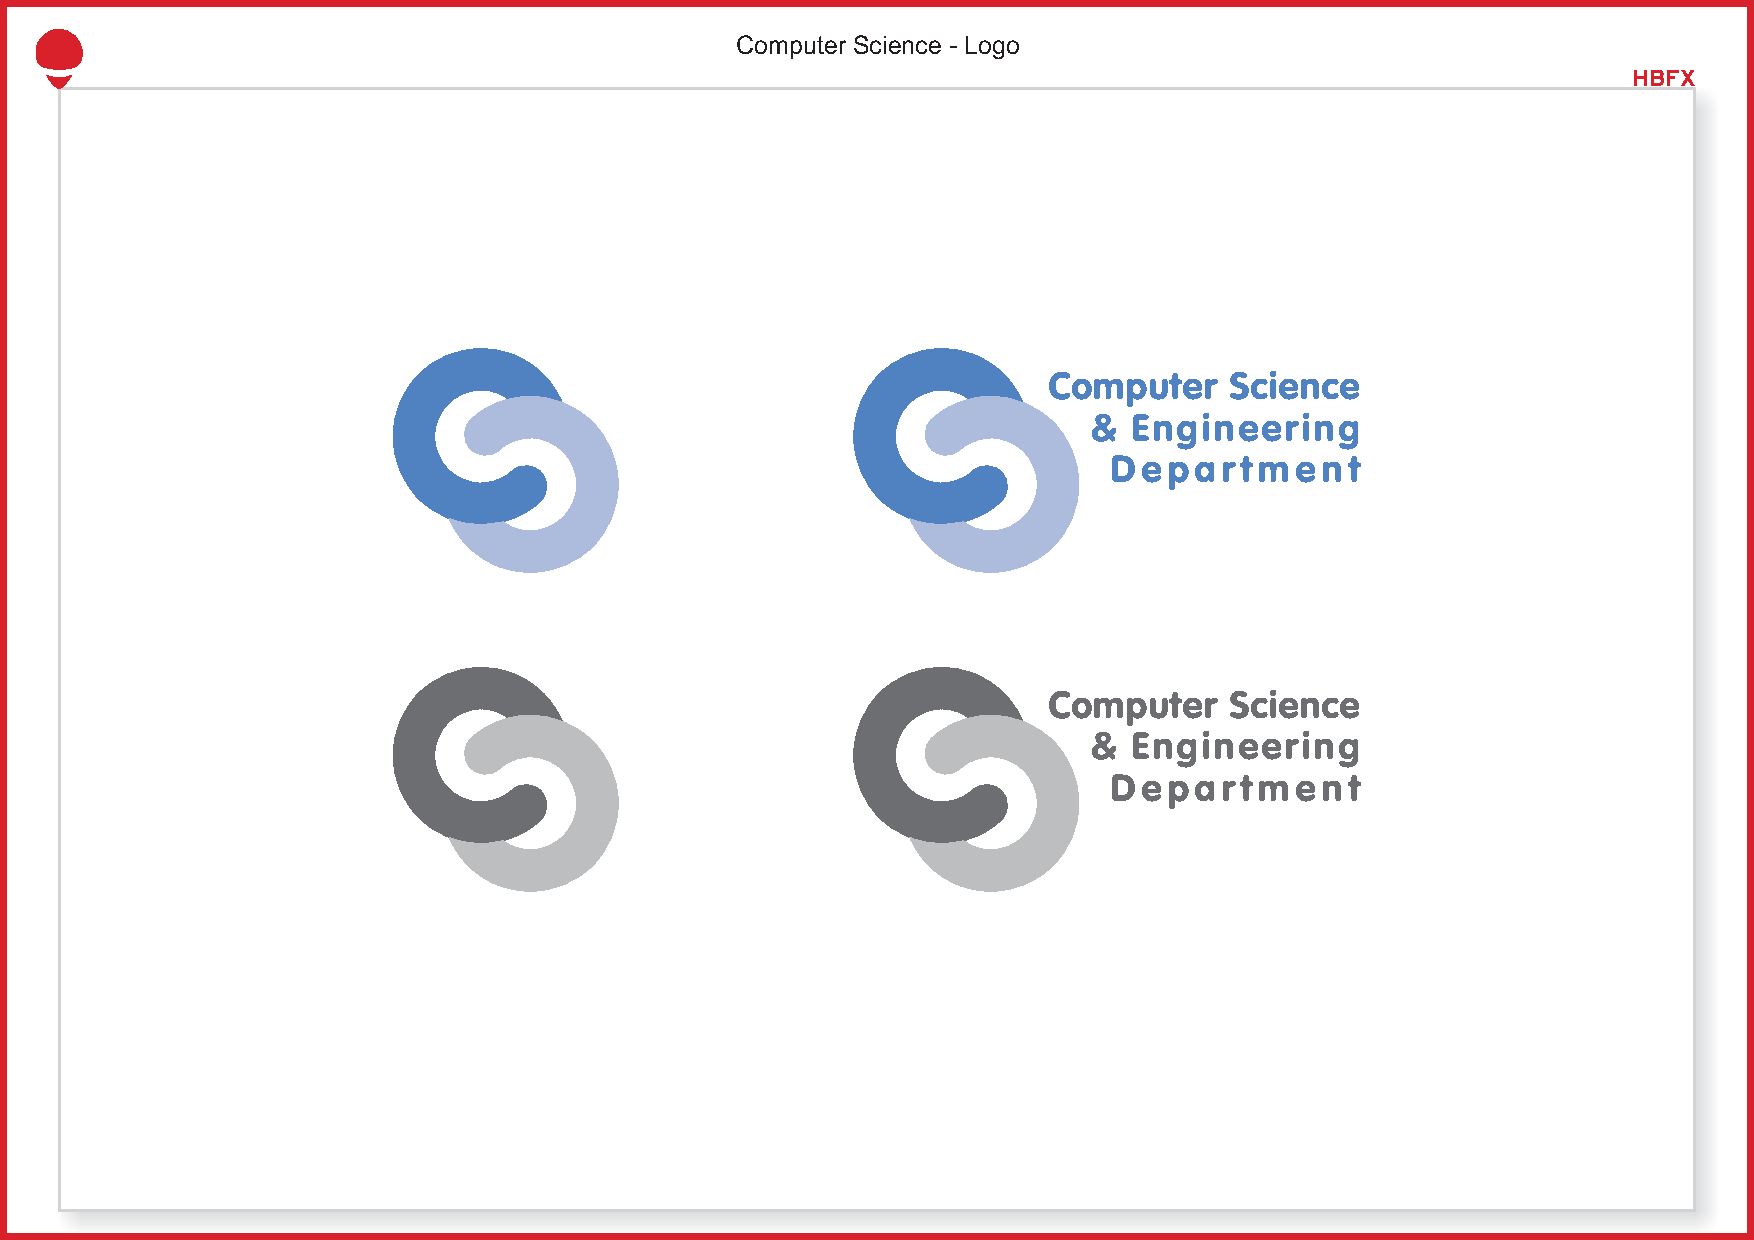
\includegraphics[scale=0.5,trim={14cm 11cm 2cm 5cm},clip=true]{pics/cs-logo.pdf}
\end{tabular}

\vspace{105pt}
{\Huge #2}\\                           % diploma project text
\vspace{40pt}
{\Large #3}\\ \vspace{0pt}  % project title
{\Large #4}\\                          % project subtitle
\vspace{40pt}
{\LARGE \Name}\\                   % student name
\end{center}
\vspace{60pt}
\begin{tabular*}{\textwidth}{@{\extracolsep{\fill}}p{6cm}r}
&{\large\textbf{#5}}\vspace{10pt}\\      % scientific advisor
&{\large \Advisor}                                    % advisor name
\end{tabular*}
\vspace{20pt}
\begin{center}
{\large\textbf{#6}}\\                                % bucharest
\vspace{0pt}
{\normalsize \Year}
\end{center}
\end{titlepage}
}

\newcommand{\frontPageRO}{\frontPage{\UniTextRO}{\DiplomaRO}{\ProjectTitleRO}{\ProjectSubtitleRO}{\AdvisorRO}{\BucRO}}
\newcommand{\frontPageEN}{\frontPage{\UniTextEN}{\DiplomaEN}{\ProjectTitleEN}{\ProjectSubtitleEN}{\AdvisorEN}{\BucEN}}

\linespread{1.15}
\setlength\parindent{0pt}
\setlength\parskip{.28cm}

%% Abstract macro
\newcommand{\AbstractPage}{
\begin{titlepage}
\textbf{\large REZUMAT}\par
\AbstractRO\par\vfill
\textbf{\large ABSTRACT}\par
\AbstractEN \vfill
\end{titlepage}
}

%% Thank you macro
\newcommand{\ThanksPage}{
\begin{titlepage}
{\noindent \large\textbf{MULȚUMIRI}}\\
\Thanks
\end{titlepage}
}



%%%%%%%%%%%%%%%%%%%%%%%%%%%%%%%%%%%%%%%%%%%%%%%%%%
%%
%%          End of template definitions
%%
%%%%%%%%%%%%%%%%%%%%%%%%%%%%%%%%%%%%%%%%%%%%%%%%%%

%%
%%   Campurile de mai jos trebuie modificate de autor. Modificati doar continutul, nu si numele fiecarei definitii
%%
\newcommand{\ProjectTitleRO}{Identificarea referințelor lipsă din lucrări științifice}
\newcommand{\ProjectSubtitleRO}{\hspace{1cm}}
\newcommand{\ProjectTitleEN}{Identifying Missing References in Scientific Papers}
\newcommand{\ProjectSubtitleEN}{\hspace{1cm}}
\newcommand{\Name}{Adrian-George Dumitrache}
\newcommand{\Advisor}{Conf. dr. ing. Costin-Gabriel Chiru}
\newcommand{\Year}{2025}

% Setări document
\title{Proiect de diplomă}
\author{\Name}
\date{\Year}

%%
%%   Campurile aferente rezumatului
%%
\newcommand{\AbstractRO}{Lucrările științifice folosesc citări pentru a oferi un context clar al literaturii relevante, pentru a își compara rezultatele cu alte lucrări, pentru a își defini poziția față de alte soluții, cât și pentru a acorda credit lucrărilor care au avut o influență directă asupra inovării lor. Totuși, natura manuală a procesului de citare poate duce la greșeli neintenționate, rezultând în citări incomplete ce subminează încrederea academica și provoacă confuzie. Detectarea acestor erori este dificilă și consumatoare de timp atât pentru autor, cât și pentru recenzori, ceea ce face automatizarea acestei sarcini extrem de utilă. Această lucrare analizează diverse metode pentru mitigarea problemei citărilor lipsă și propune un sistem complet de învățare automată pentru identificarea pasajelor ce necesită citare, împreună cu lucrările ce ar trebui citate în pasajele respective. În plus, soluția noastră este ușor de intregrat în alte aplicații ce necesită verificare automată a integrității academice, datorită faptului că avem o singură intrare simplă (lucrarea țintă), fară a avea nevoie de feedback uman suplimentar.}

\newcommand{\AbstractEN}{Scientific papers use citations to offer accurate context of the relevant literature, compare their results to other research, define their stance to current solutions, as well as to credit the works that directly influenced their innovation. However, the manual nature of citing can lead to unintentional mistakes, resulting in incomplete citations that break academic trust and cause confusion. Detecting these errors is difficult and time consuming for the author and peer reviewers alike, making automation of this task valuable. This paper analyzes various methods for mitigating missing citations and proposes an end-to-end machine learning pipeline for identifying passages where a citation is required, as well as the paper(s) that should be cited in the respective passages. Additionally, our solution is easy to integrate in other applications that require automated verification of academic integrity due to its simple input (the target paper) and no additional human feedback being required.}

%%
%%   Campurile aferente paginii de multumiri
%%
\newcommand{\Thanks}{(opțional) Aici puteți introduce o secțiunea specială de mulțumiri / acknowledgments. }

\begin{document}

\frontPageRO
\frontPageEN

\AbstractPage

\begingroup
\linespread{1}
\tableofcontents
\endgroup



% % poate fi comentata sau stearsa
% \ThanksPage


% Textul licentei incepe de aici 
\chapter{Introduction}\pagestyle{fancy}

% În cadrul introducerii, este necesară abordarea următoarelor puncte care reprezintă de fapt familiarizarea cititorului (comisia, alți colegi sau experți în domeniu) cu tema proiectului, soluția propusa și cuprinsul/structura lucrării. Deși introducerea poate conține și unele elemente mai generale, se recomandă păstrarea unui limbaj tehnic, specific audienței care va citi lucrarea.

New research always builds upon already existing publications to formulate new ideas and conclusions. However, fully explaining each concept that was borrowed from the literature takes a lot of time and can even annoy already familiar readers; this is why citing other works is the main method to mark knowledge that is not part of the author's contribution, but important to it. Citing allows authors to credit other works without redundancy, to place their work in a specific academic context, and to compare results efficiently. They are also helpful for readers, empowering them to absorb any background knowledge that is necessary for understanding a paper as they need it.

Through acknowledging prior works, researchers can develop new ideas in a structured and easy-to-follow way, placing their findings in the ever-expanding \cite{increasing-yearly-publications} graph of citations. Analysis of this graph is helpful when researching specific topics, allowing readers to get an accurate timeline of developments, but can also be used for machine learning tasks using graph based models such as Graph Neural Networks \cite{Scarselli2009TheGN} and Graph Transformers \cite{Yun2019GraphTN}.

Citations have also become an important metric for academic careers, especially as publishing has almost entirely digitized with platforms like Google Scholar\footnote{\url{https://scholar.google.com/}} or Web of Science\footnote{\url{https://www.webofscience.com/wos/}}, making summing up one's career through a simple "citation count" fairly easy. This count has led to a general "publish or perish" \cite{Mackay1974PublishOP} attitude in academia with more and more people focusing on metrics to boost their scientific career, to the dismay of some \cite{Rawat2014PublishOP} that claim this phenomenon has lead to lower quality publications, flooding the publishing space.

Unfortunately, citation is an error prone exercise. As more and more papers are being published \cite{increasing-yearly-publications}, it is becoming increasingly hard to cite correctly, as well as keep up to date with new research. Lin et al. \cite{Lin2022DetectingAA} have shown that a large number of well-accepted publications contain missing citations of named scientific entities, meaning they make basic mistakes such as mentioning the name of a machine learning model, a dataset, or an algorithm, but forget to cite the papers that introduced them. It is likely that this issue is even more prevalent outside of simple examples such as this.

Therefore, maintaining a high standard when it comes to citing is important, but is hardly trivial. The author in particular can often find it hard to assess their citations objectively. A common solution is the peer review process, which invites other researchers to read the paper and potentially identify missing citations manually. This can help catch a lot of mistakes, but is time consuming for the reviewers, making it a scarce resource.

As a consequence, automation of this task is highly valuable and can improve the academic experience for both writers and peer reviewers. In this paper, we will explore various methods for detecting missing references in scientific papers, as well as present an end-to-end pipeline for missing citation detection and retrieval. Compared to other existing solutions, ours avoids training on specific papers, performing retrieval on indexed documents. This allows for easier scalability to a wider range of published works.

\section{Context}
% O scurtă introducere a proiectului, motivație, explicație de ce este relevant domeniul proiectului.

Maintaining good citation practices is an error prone process that can be improved though computer assistance. The simple marking of sentences with "citation needed" can help writers improve the integrity of their papers by giving them direction when verifying their works, while paper recommendations can help authors find quality sources for their statements. This project aims to offer such a system, which can be later integrated into text editors, peer review platforms or academic integrity pipelines.

\section{Problem Statement} \label{problem_statement}
% Care este problema pe care proiectul o va rezolva.

Our problem can be defined as follows: 

\begin{quote}
\textit{Given scientific text, return sentences whose contents require citations, as well as an associated list of papers that could be cited in that context.}
\end{quote}

While not the only valid perspective, this problem naturally breaks down into two parts:

\begin{enumerate}
    \item Find sentences that don't seem to give enough context for their statements.
    \item Retrieve candidate papers to cite for each sentence. 
\end{enumerate}

Our solution is modeled after these natural steps, allowing us to solve the problem in a more decoupled manner. Further sections will discuss our approach incrementally, as well as alternative interpretations that solve this problem as a unified task.

\section{Objectives} \label{objectives}
% Care sunt obiectivele proiectului/soluției/abordării/ideii; Ce creșteri sau evoluții determină rezolvarea proiectului.

Our main goals for this project are offering a scalable, reliable and fast system for missing reference identification that is easy to integrate into other projects that require academic integrity verification. In pursuing these goals we will attempt to improve on the current state-of-the-art.

Because the world of academic publishing moves incredibly fast, our solution needs to be capable of adapting to a large and growing number of papers which can be recommended. This is because designing and building a solution that is only capable of recommending a well defined set of papers, either due to training or architecture constraints, will naturally become obsolete as more papers come out.

Speed is also fairly key here, as integrating a slow system into interactive applications such as text editors can vastly degrade the original experience. Ideally, we'll achieve this without losing out on performance compared to state-of-the-art solutions, but some tradeoffs are acceptable.

\section{Proposed Solution} 

Our solution is modeled after the steps proposed in section \ref{problem_statement}. The steps of our pipeline are as follows:

\begin{enumerate}
    \item To identify sentences with missing references, we use a text classifier to classify each sentence of the target paper as either citing or non-citing. Only citing sentences progress to the next step of the pipeline.
    \item For each citing sentence, we perform a fast retrieval of a set of \(k=50\) candidate papers from a database of paper titles and abstracts. The retrieval is based on semantic similarity between the statement coupled with a natural language description of the task at hand and the cited paper text.
    \item Every list of candidate papers is re-ranked using a slower, but more effective ranking method to improve the order quality. Only the top \(h=5\) results from the re-ranked lists are kept and proposed as references that could be cited for the given statements.
\end{enumerate} 

At a high level, it is simply a combination between specialized classification used to identify potential queries that are then used to perform information retrieval on a knowledge base using a method that is reminiscent of retrieval-augmented generation \cite{Lewis2020RetrievalAugmentedGF} style approaches.

This approach allows our system to scale to a larger number of papers that can be offered as candidates, as expanding the knowledge base simply involves indexing more papers. This is way more flexible compared to neural network \cite{Jeong2019ACC} or topic modeling approaches \cite{He2010ContextawareCR} which need to be re-trained if the set of possible recommendations changes.

Other citation recommendation systems \cite{He2010ContextawareCR} also require additional user input, such as manually pointing out passages with missing citations or placing placeholder citation markers. Our solution doesn't require any additional input from the user besides the target paper, making integration fairly simple.

\section{Results}
% Descriere pe scurt a rezultatelor obținute, eventual de ce acestea sunt importante față de alte soluții sau studii.

We present an end-to-end pipeline based on machine learning and information retrieval solutions that can help authors identify missing citations in their papers by identifying sentences that require citation, as well as recommending possible sources. This can be done with no additional human input besides the paper itself, making it easy to integrate in other applications.

By building upon existing works, models, and methods extracted from the literature, each step of the pipeline brings improvements leading to better overall performance or usability. In short, our solution can:

\begin{itemize}
    \item identify text that requires citation with a \textbf{10 point F1-score improvement} over the current state-of-the-art model \cite{Wright2021CiteWorthCD} by leveraging a fine-tuned large language model
    \item recommend papers to cite with a \textbf{0.5 Recall@5} while maintaining flexibility regarding the set of papers that can be recommended using semantic similarity search and re-ranking
    \item achieve high quality recommendations by combining two machine learning tasks that are traditionally studied separately (citing sentence classification \cite{Sugiyama2010IdentifyingCS} and citation recommendation \cite{He2010ContextawareCR})
\end{itemize}

Therefore, our pipeline is a high performance all-in-one solution for missing reference identification which has the potential to help researchers write higher quality papers by detecting their citation related mistakes automatically and offering insights that can help them alleviate the issues.

\section{Paper Structure}
% Un paragraf în care fiecare dintre secțiunile următoare este prezentată în 1-2 fraze, punând accentul pe elementele cele mai semnificative din fiecare secțiune.

Moving forward, we will deeply evaluate the need for our work in \autoref{motivation}, \textit{Motivation}, exploring the different ways in which scientists fail to use citations correctly.

In \autoref{sota}, \textit{State of the Art}, we'll investigate existing models and methods that solve tasks adjacent to our work. More specifically, we'll explore literature related to citing sentence detection \cite{Sugiyama2010IdentifyingCS} and citation recommendation \cite{He2010ContextawareCR}.

Then, \autoref{experiments}, \textit{Experiments}, will touch on various failed experiments that did not end up being directly part of our final solution. This chapter will clarify the chains of thought that led us to the most influential ideas behind the other, more successful, experiments. 

Chapter \ref{solution}, \textit{Proposed Solution}, will offer a high level overview of our architecture and explain each step of our solution, while \autoref{details}, \textit{Implementation Details}, will dive deeper into the technologies, code and methods that are used to power the system.

Finally, \autoref{evaluation}, \textit{Evaluation}, will deeply explore the performance of our solution by different metrics, as well as compare it to existing solutions.

\chapter{Motivation} \label{motivation}
% \cercetare Acest capitol va introduce motivația realizării proiectului propus.

% Dacă proiectul de licență face parte dintr-un proiect mai amplu (de exemplu un proiect complex, la care lucrează 2 studenți (ex: 1 student la front-end-ul aplicației, 1 student la back-end-ul aplicației), în acest capitol va fi explicat pe scurt ansamblul proiectului și ce parte din proiect este adresată de lucrarea propusă. 

% Criterii pentru calificativul \textit{Bine}: 
% \begin{itemize}
% 	\item	 \cercetare Motivația este legata de o necesitate științifica / tehnica explicită.
% \end{itemize}

Learning how to properly cite other works is a complicated process that is easy to get wrong. This is especially true for junior researchers or students, who are often more focused on delivering their contribution, as opposed to presenting their work in the scientific context in which it was developed, leading to hard to decipher arguments.

A common problem is authors considering popular and established concepts to be familiar to all readers. While this is a valid opinion, it is definitely not an excuse for not citing the works that introduced those concepts in the first place. This assumption of over-familiarity damages the integrity of the paper and the quality of the global citation graph.

Publications whose findings are now taught in university level courses are particularly vulnerable to this, as authors might have a deep understanding of the subject without having ever read the original paper. For example, perceptrons \cite{Rosenblatt1958ThePA} are a core machine learning concept that a lot of people learn about from introductory undergraduate-level courses\footnote{\url{https://openlearninglibrary.mit.edu/courses/course-v1:MITx+6.036+1T2019/course/} accessed on 30th April 2025}\textsuperscript{,}\footnote{\url{https://cs229.stanford.edu/} accessed on 30th April 2025} without being exposed to the source paper, making it likely that they'll take them for granted in their explanations.

Furthermore, named entities like websites, libraries, datasets, models etc. may or may not have associated papers which need to be cited. For instance: the HuggingFace Transformers library has an associated paper \cite{Wolf2019HuggingFacesTS}, but the most popular HTTP requests library\footnote{\url{https://requests.readthedocs.io/en/latest/}} for Python\footnote{\url{https://www.python.org/}} does not. Research by Lin et al. \cite{Lin2022DetectingAA} has shown that a large number of papers make this mistake, with some not even including links as a footnote. 

Of course, there are also simple human errors. Authors can just forget to correctly mark their citations even if they are perfectly aware of the works that they sourced from. At a large scale, mistakes are inevitable \cite{Reason2000HumanEM} due to limited human performance, errors are therefore expected no matter how banal they are, especially considering the recent increasing rate of academic research \cite{increasing-yearly-publications}.

As we can see, a lot of the mistakes that scientists make are pretty basic, coming from a lack of knowledge of the literature or human error. It is our hypothesis that these two shortcomings can be mitigated using computer assistance in the form of knowledge retrieval systems \cite{Lewis2020RetrievalAugmentedGF} and specialized machine learning models, offering a valuable tool for researchers. Of course, it's likely that very complicated cases of missing citations that require advanced reasoning exist, but the goal of this paper will be to make sure that the aforementioned common patterns will be resolved.

Taking all arguments into account, the study of methods for detecting missing citations solves a harmful problem that poisons the academic community and can help researchers write better publications, save time during peer review, and correctly credit their peers. 

\chapter{State of the Art} \label{sota}
% \cercetare Metode existente (sau ``State of the Art'') se referă, de regulă, la nivelul curent de dezvoltare: care este starea curentă a domeniului, unde ne găsim, care este contextul. Care sunt soluțiile actuale prezente în literatura de specialitate și care sunt limitările lor? Ce direcții de explorare sunt recomandate în literatura de specialitate? Literatura de specialitate se refera la articole științifice recente, publicate în reviste cu factor de impact mare, sau în volumele unor conferințe de top, sau în cărți.

% \ambele În încheierea acestui capitol se dorește descrierea tehnologiilor folosite în lucrare, cu alternative și cu argumente convingătoare calitative și cantitative.  

% Criterii pentru calificativul \textit{Bine}:
% \begin{itemize}
% 	\item \cercetare analiza literaturii de specialitate din lume, cu poziționarea precisă a lucrării în peisajul actual al domeniului studiat; 
% 	\item \ambele Sunt descrise tehnologii alternative. Sunt analizate cantitativ și calitativ, folosite benchmarkuri și teste efectuate de student. Analiza este rezumată prin tabele și grafice.
% \end{itemize}

Understanding the nature of citations has become an important sub-area of research on scholarly documents through tasks such as citation intent classification \cite{Cohan2019StructuralSF} or named entity recognition \cite{luan-etal-2018-multi}. These developments are somewhat fueled by the rise of models and systems that use citations as an input to build models that understand the relations between documents \cite{caciularu-etal-2021-cdlm-cross}, improve retrieval systems \cite{lala2023paperqa}, or analyze the evolution of an entire field of study \cite{Jurgens2018MeasuringTE}.

Our end goal of automatically detecting passages where citation is needed and recommending papers to back up those passages is most similar to the following two tasks:
\begin{enumerate}
    \item \textbf{Citing Sentence Classification} (also known as \textbf{Cite-Worthiness Detection}), introduced by Sugiyama et al. \cite{Sugiyama2010IdentifyingCS} (and later re-coined by Wright et al. \cite{Wright2021CiteWorthCD}), is the task of classifying sentences as either citing or non-citing, meaning whether a passage contains references to other works or not. This is done without the aid of reference markers (e.g: [1], [1, 2, 3], [1-5], Dumitrache et al. etc.).
    \item \textbf{Citation Recommendation} is the task of recommending papers to cite based on a target paper. It is often categorized by the context used for recommendation:
    \begin{enumerate}
        \item \textbf{Global Citation Recommendation}, introduced by Strohman et al. \cite{Strohman2007RecommendingCF}, uses only the title and abstract of a paper (known as the global context) to recommend references to add to the bibliography.
        \item \textbf{Local Citation Recommendation}, introduced by He et al. \cite{He2010ContextawareCR}, is the task of recommending citations based on the location of citation marker placeholder, as well as its surrounding text (called a local context). This method sometimes uses the global context as an extra input.
    \end{enumerate}
\end{enumerate}

In the following sub-sections, we will be discussing and evaluating each of the previously discussed concepts in detail, identify shortcomings, as well as propose ideas for improvement and paths to follow in our experimentation.

Additionally, we will explore a novel method of citation recommendation specifically designed for scientific entities that leverages a statistical approach, stepping out of the machine learning realm that most existing solutions reside in.

\newpage

\section{Citing Sentence Classification}

The task of citing sentence classification has only been studied as a supervised machine learning problem, as in taking a model architecture and training it on sentences labeled as citing or non-citing. Datasets for this task are mostly generated from large corpora of scholarly text labeled automatically using existing reference markers, which are then removed.

There are three main publications tackling this problem, each of them making subsequent improvements related to the model architecture used, as well as the quality of the dataset. We will discuss these in chronological order.

\subsection{Support Vector Machines and a Basic Corpus}

Sugiyama et al. \cite{Sugiyama2010IdentifyingCS} used SVMs (Support Vector Machines) \cite{Vapni2000TheNO} on a dataset built on the ACL Anthology Reference Corpus \cite{Bird2008TheAA}. To label sentences, they used regular expressions to detect reference markers and removed them afterwards without any extra heuristics.
    
Unfortunately, the exact methods used to generate their dataset were not provided, but we do know that it is highly imbalanced (approximately 90/10 split between non-citing and citing sentences) and likely has problems such as sentences losing their correctness after removing reference markers. The authors also fail to acknowledge that accuracy is an irrelevant metric given the imbalance in labels (e.g: 0.9 accuracy can be achieved by simply marking everything as non-citing), no mentions of other metrics such as precision, recall or F1-score exist.

Therefore, while their work is an important stepping stone, it will not be included in further comparisons, mostly due to lack of support in reproducing their results and the fact that further work \cite{Frber2018ToCO} proves that SVMs \cite{Vapni2000TheNO} are outpaced by more modern alternatives for this task.

\subsection{Recurrent Convolutional Neural Networks with an Extended Corpus}

Färber et al. \cite{Frber2018ToCO} leveraged a recurrent convolutional neural network architecture and an extended corpus of scholarly documents compared to previous work to improve results by all relevant metrics.

Their corpus \cite{Frber2018AHG} is an extension of the previously discussed one. Methods for reproducing the labeled dataset were not provided, but the description offered leads us to believe only detection and removal was performed. It suffers from the same problems of class imbalance, but uses over- and under- sampling to improve results in both their baseline SVM and RCNN model.

In the end, its results vastly outpace SVM based solutions with a 0.5 F1-score for the RCNN approach, compared to a range of 0.03-0.15 F1-score among all SVM variants.

\subsection{Transformers, Paragraph-Level Context and an Improved Method for Labeling Scholarly Text}\label{citeworth}

Wright et al. \cite{Wright2021CiteWorthCD} propose CiteWorth, a high quality dataset based on the extremely large (around 80 million papers) S2ORC \cite{Lo2020S2ORCTS} corpus, leveraging its high quality and detailed citation contexts. To ensure that the dataset maintains a high standard of quality, in addition to detecting reference markers and removing them, it also employs heuristics to:

\begin{enumerate}
    \item Ignore samples where removing reference markers would break grammar, e.g: "As shown by [1, 2, 3]" is an incomplete sentence without the reference markers and, thus, it would be ignored.
    \item Ignore samples that are detected as having reference markers despite S2ORC not marking them as such.
    \item Only include sentences that are at least 20 characters long.
    \item Only include sentences that follow basic conventions (capital letter, ended with normal punctuation etc.).
\end{enumerate}

They also employ manual human evaluation to compare these heuristics to a baseline detect-and-remove method, proving it leads to a higher quality dataset.

CiteWorth \cite{Wright2021CiteWorthCD} also groups all sentences by paragraph and only takes into consideration paragraphs whose sentences respect the aforementioned rules. This is done to easily incorporate the larger context of a sentence in its classification. An intuition for why this could be helpful can be developed through the following paragraph extracted from the SciBERT paper \cite{beltagy2019scibertpretrainedlanguagemodel}:

\begin{quote}
    \textit{The BERT model architecture (Devlin et al., 2019) is based on a multilayer bidirectional Transformer (Vaswani et al., 2017). Instead of the traditional left-to-right language modeling objective, BERT is trained on two tasks: predicting randomly masked tokens and predicting whether two sentences follow each other. SCIBERT follows the same architecture as BERT but is instead pretrained on scientific text.}
\end{quote}

As we can see, the first mention of BERT \cite{devlin2019bertpretrainingdeepbidirectional} in the paragraph cites the paper that introduced the model, but later mentions do not. This is fairly common behavior for most authors, but can be misleading when training a model at the sentence level.

Next, the authors fine-tune various pre-trained Transformer \cite{vaswani2023attentionneed} models, with the most successful being SciBERT \cite{beltagy2019scibertpretrainedlanguagemodel} for sentence level classification and Longformer \cite{beltagy2020longformerlongdocumenttransformer} for classifying sentences in the context of their paragraphs. 

The resulting models have better metrics than the previous ones, at 0.62 F1-score for single-sentence classification and 0.67 for multi-sentence/paragraph-level classification.

\subsection{Comparison and Moving Forward}

As seen in Table~\ref{tab:citsent-metrics}, the Longformer-based \cite{beltagy2020longformerlongdocumenttransformer} model outperforms all other options, making it the current documented best model for this specific task. It is also a model that is fairly reasonable to run on local, consumer-grade hardware, making it perfect for integration into various tools.

\begin{table}[th]
\centering
\small
\setlength{\tabcolsep}{12pt}
\renewcommand{\arraystretch}{1.2}
\begin{tabular}{lccc}
\toprule
\textbf{Model} & \textbf{Precision} & \textbf{Recall} & \textbf{F1-score} \\
\midrule
RCNN & 49.57 & 65.56 & 56.41 \\
SciBERT & 57.03 & 68.08 & 62.06 \\
Longformer & \textbf{59.92} & \textbf{77.15} & \textbf{67.45} \\
\bottomrule
\end{tabular}
\caption{Performance metrics for different SOTA models on citing sentence classification using the CiteWorth dataset, all weighted}
\label{tab:citsent-metrics}
\end{table}

This leads us to the hypothesis that we could improve performance even more by looking at sentences in a larger context or, at least, using full attention instead of sparse attention at the paragraph level. Since the release of the papers discussed so far, we have seen the rise of large language models with larger and larger context windows \cite{Achiam2023GPT4TR,Reid2024Gemini1U}, leading us to ask: what if we used them as citing sentence classifiers? This idea will be explored in further chapters.

\section{Citation Recommendation}

The task of citation recommendation involves offering a list of candidate papers to cite based on a target paper as input. It has been approached from multiple angles, but many of the existing approaches are not a good fit for our use case.

\subsection{Using Global Context}

The global citation recommendation \cite{Strohman2007RecommendingCF} task boils down to recommending papers to include in the bibliography based solely on the title and abstract of the target paper. While this mostly works if we are simply interested in seeing what the most similar papers look like, it is a way less focused approach that doesn't give enough information regarding why a paper should be cited.

Since we are interested in finding missing citations based on actual statements made in the content of the paper that users can assess, we can safely ignore this type of citation recommendation.

\subsection{Using Local Context}

The local citation recommendation \cite{He2010ContextawareCR} task uses a specific context (some text) with a placeholder citation marker to recommend citations. This placeholder mostly stems from the fact that these systems only focus on recommending citations, often considering the previously discussed task of citing sentence detection as solved or proposing users to input the model with sentences manually. Our work will do without them.

Actual implementations vary in approach, using models such as topic modeling \cite{He2010ContextawareCR} or neural networks \cite{Tang2014CrosslanguageCC, Ebesu2017NeuralCN}. While these approaches exhibit fairly decent results, they unfortunately have scalability issues when it comes to extending the number of papers that can be recommended by the model, requiring re-training whenever new publications have to be added.

This makes these models quite unwieldy for real-life scenarios as they constantly require compute effort to re-train due to new papers coming out at an increasing rate \cite{increasing-yearly-publications}. Due to these issues, we will pursue the design of a new local citation recommendation model.

\subsection{Next Steps}

Local citation recommendation mostly describes what we're looking for, but current approaches are not viable given the objectives we defined in \autoref{objectives}, meaning that current solutions aren't flexible enough to support an evolving set of papers.

Since this is a very knowledge-intensive task, we propose exploring retrieval-augmented generation \cite{Lewis2020RetrievalAugmentedGF} style methods for retrieving papers relevant to a target context. This type of retrieval system only requires indexing new papers through text embeddings, solving our scalability problem. This will be explored in more detail in the following sections.

\section{Scientific Entity Recognition and Recommendation}

While most solution for detecting missing citations and recommending references rely on sub-symbolic representations of the problem to achieve their results, Lin et al. \cite{Lin2022DetectingAA} propose a natural language processing method based on the detection of scientific entities, a special case of named entity recognition \cite{Lample2016NeuralAF} that focuses on detecting terms that represent concepts published in scientific papers.

This method uses the number of co-occurrences between recognized scientific entities and citations in the same sentence to map concepts to their source papers. These mappings are generated statistically by computing co-occurrences on the S2ORC dataset \cite{Lo2020S2ORCTS}, a large corpus of scientific papers, and can then be used for citing sentence detection and citation recommendation on target papers by marking passages that contain scientific entities as needing to cite the associated paper. 

While the proposed solution manages to solve two separate tasks simultaneously: citing sentence detection and citation recommendation, it only does so for the very specific case of missing citations of scientific entities which, as discussed in \autoref{motivation}, does not represent all cases of missing references.

This issue is also reflected by the fact that the method does not have an evaluation done on any relevant datasets, the main form of evaluation being performed by applying it on papers to discover missing citations. Therefore, with no clear path to generalizing this method to more broad use cases due to the complexity of the problem, we will focus on sub-symbolic approaches in our solution.

However, this is not to say that symbolic approaches do not have their place in this problem. Arguably, their high explainability could lead to easier to understand responses by offering the reason why a passage requires citation (uncited scientific entities, statistics/percentages without a source etc.).

\chapter{Experiments} \label{experiments}

Though they are not necessary for understanding the final proposed solution, the failed experiments outlined in this chapter present the logical set of steps that were taken in our research, each one offering us a new direction to explore. Therefore, they are important for gathering insights and developing a deep understanding of our problem.

\section{Large Language Models for Identifying Missing Citations}

LLMs have proven to be adequate for a large set of machine learning tasks without any targeted fine-tuning of the model besides a couple of example inputs/outputs \cite{brown2020languagemodelsfewshotlearners}, making them an even more convenient solution than popular transfer learning \cite{Raffel2019ExploringTL} methods. It is therefore worth our time to explore whether our problem can simply be solved through prompt engineering before implementing a specialized solution.

\subsection{General Approach}

We used the popular ChatGPT interface to evaluate GPT4 \cite{Achiam2023GPT4TR} for missing reference detection by asking it to reconstruct the bibliography of a given paper using real scientific works and backing up its choices with quotes from the paper, covering our needs of classification and retrieval described in previous sections.

We evaluated two different scenarios: a realistic version where the target paper does not have citation markers (e.g: [1], [2, 3] etc.) and a version with them included. The model was also tested on papers with very different characteristics.

The problem was described in natural language using the following prompt:

\begin{quote}
\textit{You are a highly experienced scholar that constantly reads scientific papers. I have this scientific paper text from a conference, but I lost all its references. Could you take a look and attempt to find papers that are referenced by this paper? I'm interested in the name of the paper, its authors and the reason why you think so (preferably quoting the original text). I'm only interested in papers you are 100\% sure exist.}

\textit{Please keep in mind that this paper is from a renowned scientific conference, meaning it is likely that all of its references come from academic works such as scientific journals and scientific conferences.}

\textit{I will now proceed to give you parts of the text in separate messages, as it's too long for one message. After each part, please give me information about the papers you think are cited. Keep in mind that not all excerpts I send you need to contain references, please only tell me about papers you're sure are referenced.}
\end{quote}

Our prompt is designed to describe the problem, its input, and its output, as well as reinforce the idea that we want real sources. A lot of our experiments suffered from being recommended low quality sources, usually offered by web search agentic tools integrated into the chatbot. To fix this, additional instructions are given to force the model to only consider academic works as candidates in order to avoid referencing informal articles and other unreliable sources.

The prompt features slight modifications in the scenario where citations markers are still present, adding the following sentence to the problem description: \textit{Meaning, for each "[x]" or "[x, y]" or "[x-x+n]" mark, try to figure out what papers were being cited.}.

\subsection{Testing}

We tested both scenarios on three separate papers with various characteristics:

\begin{enumerate}
    \item A paper \cite{tan2024devbenchmultimodaldevelopmentalbenchmark} still in peer review at test time\footnote{Early January, 2025} which cites a lot of cutting edge research
    \item An older, very popular paper \cite{vaswani2023attentionneed} ($\sim100k$ citations)
    \item An older, less popular paper \cite{Jiang2017UnleashingTP} ($\sim50$ citations)
\end{enumerate}

We chose these papers strategically so we can evaluate the model's performance on papers it has surely been trained on (such as paper 2), as well as on papers that it hasn't been trained on or whose findings weren't reinforced through external sources (such as paper 1 and paper 3, respectively). A comparison between the performance of the model on each paper and scenario combination can be seen in \autoref{fig:llm-experiment-percentages}.

\begin{figure}[th]
\centering
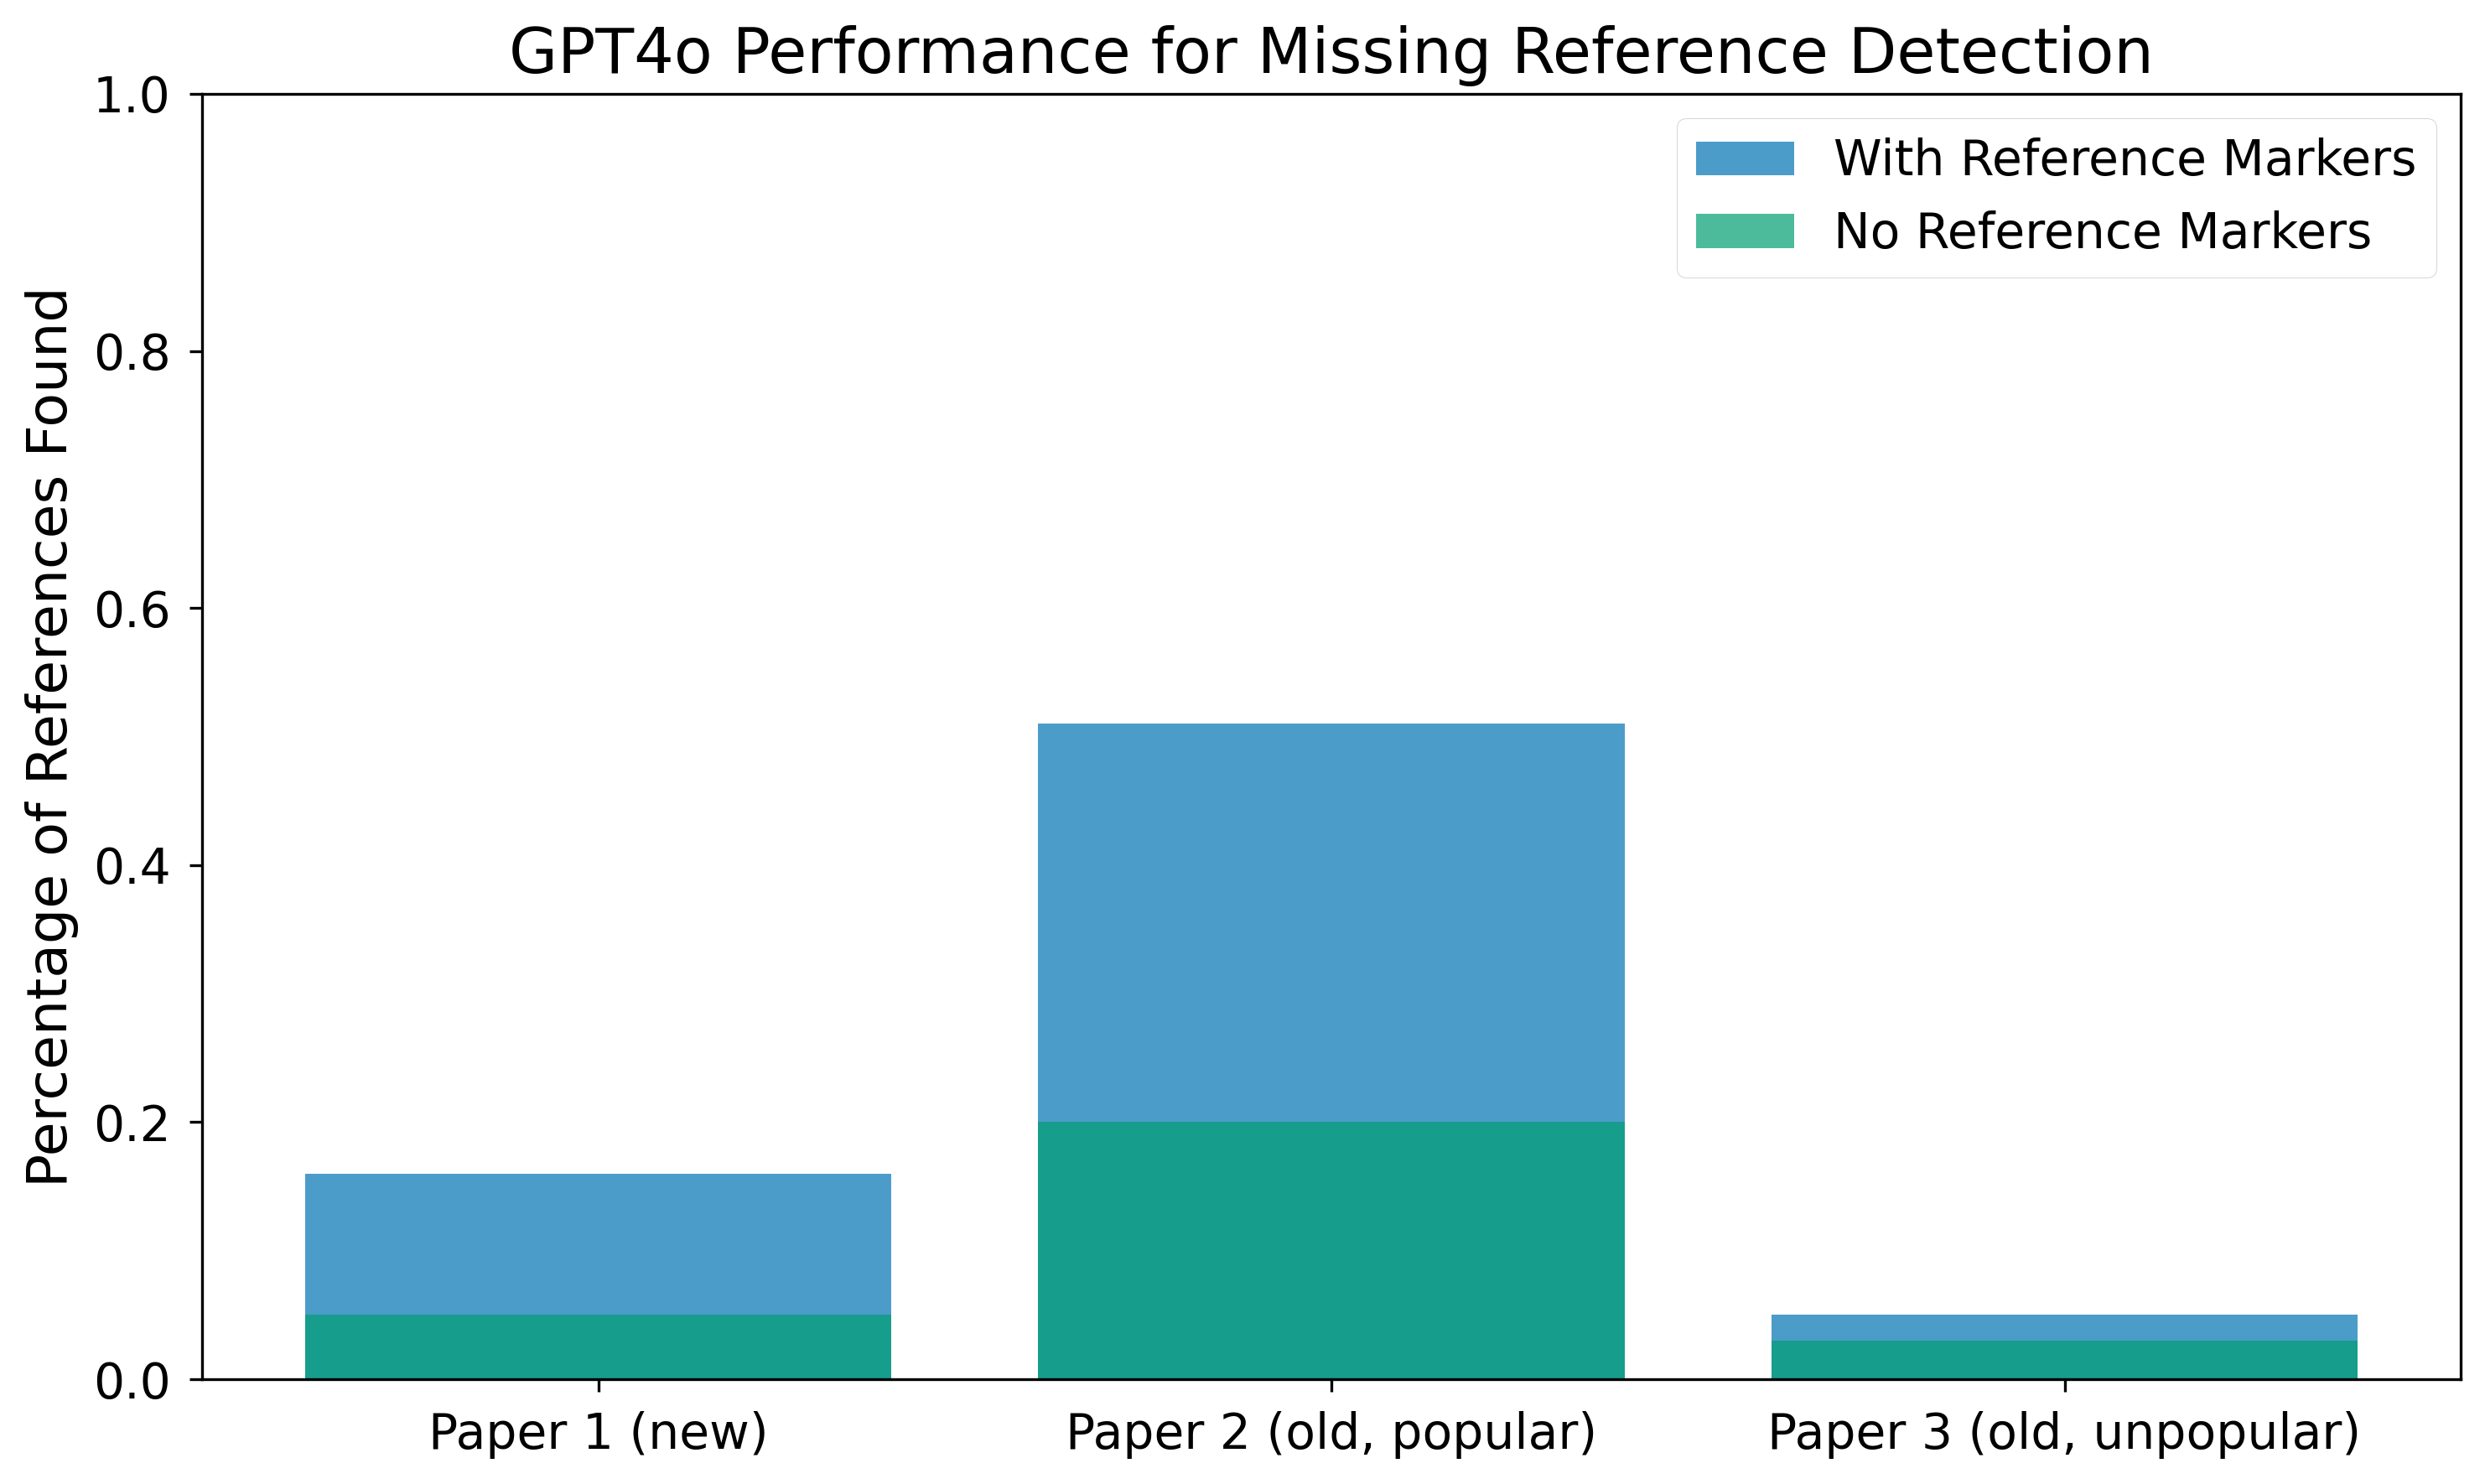
\includegraphics[width=\linewidth]{pics/gpt4o_performance_missing_reference_detection.png}
  \caption[Bar plot comparing performance of GPT4o for missing reference identification by the percentage of references identified]{Bar plot comparing performance of GPT4o for missing reference identification by the percentage of references identified}
  \label{fig:llm-experiment-percentages}
\end{figure}

Clearly, the performance is quite poor overall. Besides the weak metrics, some other issues that have come up are:

\begin{enumerate}
    \item The total number of recommendations given for scenarios with no citation markers is fairly low compared to the real number of references.
    \item Some recommendations are hallucinated \cite{Huang2023ASO} papers that do not exist.
    \item Sometimes when a correct title is offered, the wrong authors are mentioned.
    \item It is mostly unable to recommend any paper that isn't popular and fairly old. This is likely because newer, niche papers weren't used in the training set.
    \item The model often recommends the same paper as a candidate for multiple reference markers.
\end{enumerate}

\subsection{Conclusions and Next Steps}

These observations are enough to rule out the possibility that a pre-trained LLM could solve our problem without any specialized solutions (at least currently). The poor performance on a new paper and the lack of recently published candidate papers shows that our main motivation, verifying citation integrity before publishing, is not satisfied.

We can conclude that it is worth pursuing a specialized solution to our problem. Based on the issues we identified earlier, our solution will definitely need a way to ground its recommendations to a real and varied set of papers, as well as be able to detect passages that need citations with a higher accuracy. 

\section{Citation Recommendation Using Text Embeddings}

Information retrieval systems that leverage text embedding models have become popular due to their flexibility and ease of use. These models can encode text in an n-dimensional vector space, placing semantically similar sequences of text close to each other. This allows us to use metrics such as dot-product or cosine similarity to determine how semantically close two sequences of text are.

A typical architecture for such a system often involves a database of vectors that represent documents. Searches can be performed on the database by generating an embedding of the query and performing a k nearest neighbor search. This is often the basis of retrieval augmented generation systems \cite{Lewis2020RetrievalAugmentedGF}.

\subsection{Testing Scenario}

We experimented with a couple of text embedding models for retrieving paper abstracts based on a given text sequence. Our experimental setup uses a database of around \(50k\) paper abstracts randomly extracted from S2ORC \cite{Lo2020S2ORCTS} and a couple of sample passages which should cite a certain paper (which is also indexed in the database). This is done to see if the embedding model is capable of finding the correct paper among a larger pool of candidates, as opposed to just verifying the order against a couple of examples.

The passages we chose are fairly simple, often mentioning concepts which have an entire paper dedicated to them by name, an example being: \textit{"We used the Adam optimizer."}. Our goal was to filter through models fast on the premise that we probably can't get decent performance out of a model that doesn't work well on even the simplest of cases.

\subsection{Results}

Unfortunately, testing this scenario with a couple of popular text embedding models such as all-MiniLM-L6-v2\footnote{https://huggingface.co/sentence-transformers/all-MiniLM-L6-v2} and bge-m3 \cite{Chen2024BGEMM} did not produce satisfying results. None of the models managed to retrieve a single correct paper in their top 100 results, not justifying further evaluation.

This is likely due to the complexity of the task at hand, as well as the fact that the semantic characteristics of our queries and abstracts are not necessarily similar enough to warrant our high expectations. A sentence which cites a certain scientific paper does not have to be semantically similar to the abstract of the cited paper, it's more likely be closer in the vector space to other sentences which refer to the cited paper.

To alleviate this, we decided to experiment with instruction-tuned text embedding models. Their main advantage is that they allow us to describe our task in natural language, encoding text and a description of the task in a single vector. This idea ended up passing our preliminary tests, making it worth further evaluation. Our final solution now uses E5 Large Instruct \cite{Wang2024MultilingualET}, as described in \autoref{solution}.

\chapter{Proposed Solution} \label{solution}

% Capitolul conține o privire de ansamblu a soluției ce rezolvă problema, prin prezentarea structurii / arhitecturii acesteia. În funcție de tipul lucrării acest capitol poate conține diagrame (clase, distribuție, workflow, entitate-relație), demonstrații de corectitudine pentru algoritmii propuși de autor, abordări teoretice (modelare matematică), structura hardware, arhitectura aplicației.

% Criterii pentru calificativul \textit{Bine}: 
% \begin{itemize}
% 	\item 	Descriere + diagrame de baze de date, workflow, clase, algoritmi + descrierea unui proces prin care s-a realizat arhitectura/structura soluției.
% \end{itemize}

Our solution consists of a multi-step pipeline that encompasses both citing sentence detection \cite{Sugiyama2010IdentifyingCS, Frber2018ToCO, Wright2021CiteWorthCD} to identify passages with missing citations, as well as a local citation recommendation \cite{He2010ContextawareCR} system powered by retrieval based on cosine similarity of text embeddings. \autoref{fig:citation-identification-diagram} describes the entire process for a single sentence.

\begin{figure}[th]
\centering
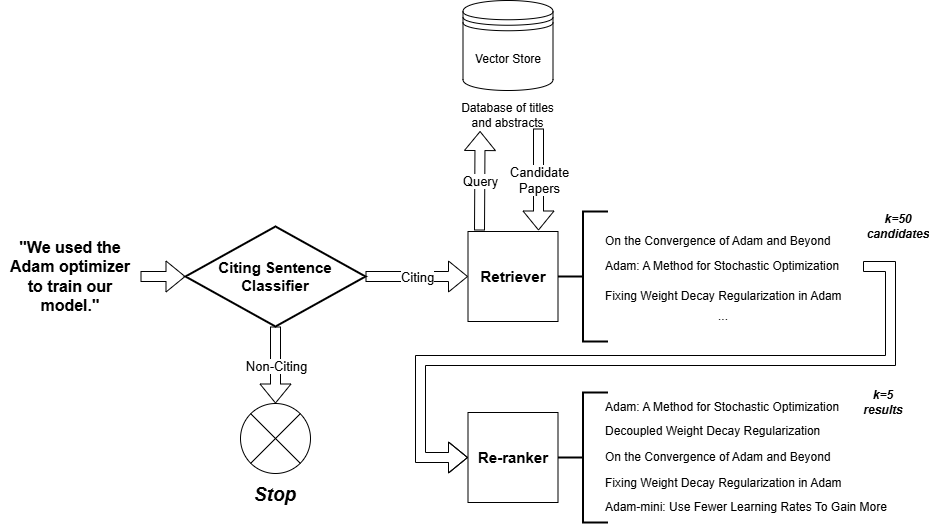
\includegraphics[width=\linewidth]{pics/citeseek_low_level_diagram.drawio.png}
  \caption[Diagram describing the process of identifying missing citations for a single sentence]{Steps for identifying missing citations for a single sentence.}
  \label{fig:citation-identification-diagram}
\end{figure}

A citing sentence classifier is used to decide whether a given sentence requires citation or not. Only sentences that need citations are passed to the retriever, which builds a query to our vector database to retrieve \(k=50\) candidate papers.

While the retriever is very fast and scales well to a large number of papers, it is not accurate. We deploy a second step to our retrieval process, which re-ranks the candidate papers using a large language model \cite{Sun2023IsCG,Sun2023InstructionDM}. This was done to balance between quality of results and time performance, offering us the best of both worlds: fast retrieval through vector search and quality ordering through LLM re-ranking.

To respect Miller's Law \cite{yablonski2020laws}, we only return the top 5 papers from the reordered list. This makes it easy for users to scan the proposed solutions quickly without getting overwhelmed.

\newpage

This pipeline can then be applied to an entire paper as input, as seen in \autoref{fig:paper-pipeline}, to offer a full report of missing citations across the document.

\begin{figure}[th]
\centering
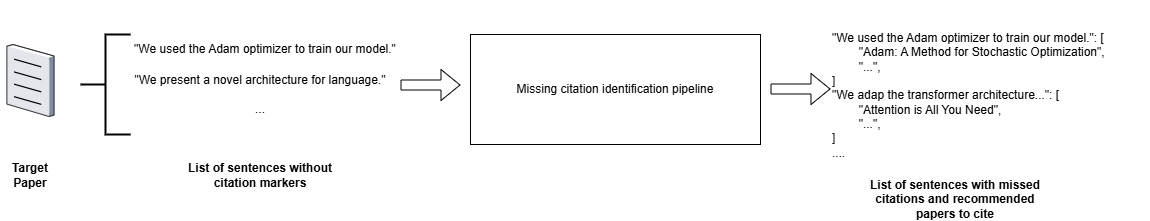
\includegraphics[width=\linewidth]{pics/citeseek_high_level_architecture.drawio.png}
  \caption[Diagram describing the process of identifying missing citations for an entire paper]{Identifying missing citations for an entire paper.}
  \label{fig:paper-pipeline}
\end{figure}

The output of our pipeline can be summarized as a list of sentences which should've used citations and associated lists of candidate papers to cite for each of those sentences. 

The following sections will describe each step of our solution in detail.

\section{Citing Sentence Detection} \label{gemini_citeworth}

We use a cite-worthiness detection model \cite{Sugiyama2010IdentifyingCS} at the paragraph level to decide which sentences require citation recommendation. As described in \autoref{citeworth}, considering the paragraph context of each sentence highly increases performance \cite{Wright2021CiteWorthCD} compared to single sentence classification, likely due to varied citation practices among researchers such as only citing a paper once per paragraph.

Our classifier model is a version of Gemini Flash 2.0 \cite{gemini-flash-2} fine-tuned on the CiteWorth dataset \cite{Wright2021CiteWorthCD} to classify sentences in the context of their paragraphs by generating a label for each sentence. We improve on the existing state-of-the-art, that being Longformer \cite{beltagy2020longformerlongdocumenttransformer} trained on the same dataset, by tackling two of its main limitations:

\begin{itemize}
    \item Longformer \cite{beltagy2020longformerlongdocumenttransformer} uses a sparse attention mechanism \cite{Child2019GeneratingLS} to handle longer passages, trading performance for a larger context window while maintaining almost the same number of parameters as models with a smaller window and full attention (such as RoBERTa \cite{Liu2019RoBERTaAR})
    \item it has a parameter count of around 100 million \cite{beltagy2020longformerlongdocumenttransformer}, a fairly low number compared to newer language models
\end{itemize}

This led us to the hypothesis that improved performance could be achieved using a language model with full attention, a large enough context window to fit a regular paragraph, as well as more parameters. LLM families such as GPT \cite{Achiam2023GPT4TR} and Gemini \cite{Reid2024Gemini1U} satisfy all of these requirements.

Even though training or fine-tuning such a model used to be out of reach for most users due to hardware constraints, services for this kind of compute have become a convenient offering of cloud platforms like Vertex AI, making it a viable option even without access to a cluster or specialized hardware.

Taking advantage of this, we fine-tuned every parameter of Gemini Flash 2.0 \cite{gemini-flash-2} in a supervised manner by training it on whole paragraphs as input and citing/non-citing labels for each sentence in each paragraph as outputs to compare to. We also add additional formatting to the inputs and reference outputs in the form of sentence number tags to make it easier for the model to count, a problem that LLMs often have a hard time solving \cite{Fu2024WhyDL}.

Details regarding the dataset used for fine-tuning, CiteWorth \cite{Wright2021CiteWorthCD}, can be seen in \autoref{tab:citeworth-stats}

\begin{table}[th]
\centering
\small
\setlength{\tabcolsep}{12pt}
\renewcommand{\arraystretch}{1.2}
\begin{tabular}{lccc}
\toprule
\textbf{Metric} & \textbf{Value} \\
\midrule
Sentence count &  1,181,793 \\
\% citing & 31.76\% \\
\% non-citing & 68.24\% \\
Train/Test/Validation split & 80/10/10 \\
Train sentences & 945,426 \\
Validation sentences &  118,182 \\
Test sentences & 118,185 \\
Scientific field coverage & 10 different fields \\
Publication years & Up to 2021 \\
\bottomrule
\end{tabular}
\caption{Statistics regarding the CiteWorth dataset \cite{Wright2021CiteWorthCD}}
\label{tab:citeworth-stats}
\end{table}

Our inputs are therefore formatted as follows:

\begin{quote}
    0: \texttt{<}sentence\texttt{>}
    
    1: \texttt{<}sentence\texttt{>}
    
    ...
    
    n: \texttt{<}sentence\texttt{>}
\end{quote}

These inputs also have associated labels which can be used to update the parameters, tuning the model:

\begin{quote}
    0: non-check-worthy/check-worthy
    
    1: non-check-worthy/check-worthy
    
    ...
    
    n: non-check-worthy/check-worthy
\end{quote}

This setup has allowed us to fine-tune the model into a generative cite-worthiness classifier that beats out the performance of the previous state-of-the-art model by all relevant metrics on the test split of CiteWorth \cite{Wright2021CiteWorthCD} (over \(100k\) sentences), gaining over 10 F1 points over it. An in-depth comparison can be found in \autoref{evaluation-citsent}.

Of course, running this model locally on most consumer-grade systems is not realistic due to its complexity, but inference in a cloud environment is fast and fairly inexpensive\footnote{Less than 1 US Dollar for inference on the entire CiteWorth test split of over \(100k\) sentences, tested through Vertex AI}, mostly due to the low number of output tokens required. It is likely that this will become even more accessible in the future, either due to capable hardware being more generally available or similar advances in cloud offerings. 

\section{Retrieval}

We use a database that stores paper titles and abstracts as vectors generated by a text embedding model, E5 Large Instruct \cite{Wang2024MultilingualET}. This model allows us to place queries (citing sentences) and relevant paper text close to each other in the vector space, allowing us to retrieve candidate papers based on the distance between vectors.

Being an instruct embedding model, we can also use natural language to describe the retrieval task at hand before offering it our query sentence, conditioning the generated embeddings on a specific task. The following description of our task is used to encode the queries:

\begin{quote} \label{quote:prompt}
    \textit{Given a sentence where a paper is cited, find the abstract of the paper it cites.}
\end{quote}

Evaluating this retrieval method on the PeerRead dataset \cite{Kang2018ADO}, a large corpus of citing sentences/contexts and papers to recommend from, results in a Recall@50 of \(0.46\). This means that for \(46\%\) of citing sentences provided by the dataset, the correct paper that should be cited appears in the \(k=50\) candidate papers.
    
A couple examples of retrieval results can be seen in \autoref{tab:retriever-examples}, showcasing some scenarios that the retriever excels at, finding scientific named entities. However, the method is sometimes limited by its usage of semantic similarity, the fourth example in \autoref{tab:retriever-examples} is a scenario in which the usage of the term \textit{Berkeley-Parser} serves as more of a hindrance since the original paper did not coin this term for their innovation, it came to be after the paper was published.

\begin{table}[th]
\centering
\small
\setlength{\tabcolsep}{10pt}
\renewcommand{\arraystretch}{1.3}
\begin{tabularx}{\linewidth}{X X c}
\toprule
\textbf{Sentence} & \textbf{Cited Paper} & \textbf{Position In Results} \\
\midrule
\textit{We used the Adam optimizer with \(\beta1 = 0.9\), \(\beta2 = 0.98\) and \(\epsilon = 10-9.\)} 
& Adam: A Method for Stochastic Optimization & 2 \\
\textit{…we replace our sinusoidal positional encoding with learned positional embeddings…}
 & Convolutional Sequence to Sequence Learning
 & 4 \\
\textit{Recent work has achieved significant improvements in computational efficiency through factorization tricks…}
 & Factorization tricks for LSTM networks
 & 3 \\
 \textit{...the Transformer outperforms the Berkeley-Parser.}
 & Learning accurate, compact, and interpretable tree annotation
 & Not found
 \\
\bottomrule
\end{tabularx}
\caption{Retrieval results on some sample sentences extracted from Vaswani et al.\cite{vaswani2023attentionneed}, retrieved from a database of around \(50k\) papers which includes each cited paper.}
\label{tab:retriever-examples}
\end{table}

\newpage

To get the closest vectors to our query vector, the database system uses a fast approximate k-nearest-neighbor algorithm to determine \(k=50\) similar vectors to our query by dot-product\footnote{Arguably, cosine similarity is used, but because we normalize our vectors, it becomes equivalent to the dot-product of the vectors.}, this allows us to comb through a large databases of embeddings and get relevant candidates without scaling linearly (an exact KNN search is \(O(n)\)).

Our model choice is based on benchmark results\footnote{\url{https://huggingface.co/spaces/mteb/leaderboard}, intfloat/multilingual-e5-large-instruct is 4th place, last accessed on 8th May 2025}, where E5 Large Instruct \cite{Wang2024MultilingualET} ranks very well. The only models that outperform it are unreasonable to use on local systems, as they can have over 14 times more parameters than E5. For reference, such a model takes around a minute to generate a single vector on a consumer GPU.

While this method does give us a relevant list fairly quickly, its order is rarely accurate even for obvious scientific named entities, as seen in \autoref{tab:retriever-examples}. The main purpose of this step is to fetch a list of likely candidates from a large database of papers in a short time. Our next step is, based on the origin of each returned vector, to construct a list of papers (title + abstract) of candidate papers that can be passed to a re-ranking step.

\section{Re-ranking}

To improve the order of our candidate papers, we employ a large language model based re-ranking method in the form of RankGPT, introduced by Sun et al. \cite{Sun2023IsCG,Sun2023InstructionDM}. RankGPT uses LLMs to rank text passages according to a given prompt by leveraging a listwise-approach for instructional permutation generation, basically using LLMs as comparison functions between passages.

The passages we will re-rank are simply the title and abstract of each paper concatenated. They will be re-ordered according to the same prompt we used for the embedding model along with the citing sentence we are targeting. This method produces quality results, almost always improving the initial list, as can be seen in \autoref{tab:reranker-examples}.

Even though RankGPT \cite{Sun2023IsCG,Sun2023InstructionDM} could be theoretically deployed as a pure retriever that outputs higher quality results without a two step process, it does not scale well to a large number of papers (even re-ranking 50 papers takes longer than the retrieval step), making it too slow to deploy at the scale of an entire database of papers, but perfect as a re-ranker.

\begin{table}[th]
\centering
\small
\setlength{\tabcolsep}{10pt}
\renewcommand{\arraystretch}{1.3}
\begin{tabularx}{\linewidth}{X X c c}
\toprule
\textbf{Sentence} & \textbf{Cited Paper} & \textbf{Initial Result} & \textbf{After Re-Rank} \\
\midrule
\textit{We used the Adam optimizer with \(\beta1 = 0.9\), \(\beta2 = 0.98\) and \(\epsilon = 10-9.\)} 
& Adam: A Method for Stochastic Optimization & 2 & 1 \\
\textit{…we replace our sinusoidal positional encoding with learned positional embeddings…}
 & Convolutional Sequence to Sequence Learning
 & 4 & 2 \\
\textit{Recent work has achieved significant improvements in computational efficiency through factorization tricks…}
 & Factorization tricks for LSTM networks
 & 3 & 1 \\
 \textit{...the Transformer outperforms the Berkeley-Parser.}
 & Learning accurate, compact, and interpretable tree annotation
 & Not found & Not Found
 \\
\bottomrule
\end{tabularx}
\caption{Re-ranking results on some sample sentences extracted from Vaswani et al.\cite{vaswani2023attentionneed}, retrieved from a database of around \(50k\) papers which includes each cited paper. Only top 5 taken into account in re-ranking results.}
\label{tab:reranker-examples}
\end{table}

The preliminary results of \autoref{tab:reranker-examples} are also backed up by a large scale evaluation performed on the PeerRead dataset \cite{Kang2018ADO}. We used our retriever to generate lists of candidates and passed them to the re-ranker. To evaluate the re-ranker fairly, we supplement the lists with the correct paper if it's not already present. This is done to prevent an analysis of the re-ranker that caps its performance to the retriever. To better illustrate this issue: if the correct paper is present only in \(40\%\) of lists, then re-rank evaluation on the other \(60\%\) is in vain, as we have no other means of evaluating quality besides the position of the cited paper.

The final result is a Recall@5 of \(0.49\) if we force the correct paper to be in the initial list, showing the independent quality of the re-ranker. 

Faster, more traditional re-ranking models such as bge-reranker-base \cite{bge_embedding} were not able to match its performance. In fact, any model that did not feature the ability to describe the task at hand in natural language has failed, even offering worse results than our retriever. 

\chapter{Implementation Details} \label{details}
% În plus fata de capitolul precedent acesta conține elemente specifice ale rezolvării problemei care au presupus dificultăți deosebite din punct de vedere tehnic. Pot fi incluse configurații, secvențe de cod, pseudo-cod, implementări ale unor algoritmi, analize ale unor date, scripturi de testare. De asemenea, poate fi detaliat modul în care au fost utilizate tehnologiile introduse in capitolul 3.

% Criterii pentru calificativul Bine: 
% 	Descrierea detaliată a algoritmilor/structurilor utilizați; Prezentarea etapizată a dezvoltării, inclusiv cu dificultăți de implementare întâmpinate, soluții descoperite; (dacă este cazul) demonstrarea corectitudinii algoritmilor utilizați. 

This chapter will zoom in on our solution to discuss the technical details that make it a good candidate for further integration into existing applications. We will touch on the provided interface, the technologies and frameworks used, small code details that improve its quality, as well as important design decisions that were taken.

\begin{figure}[th]
\centering
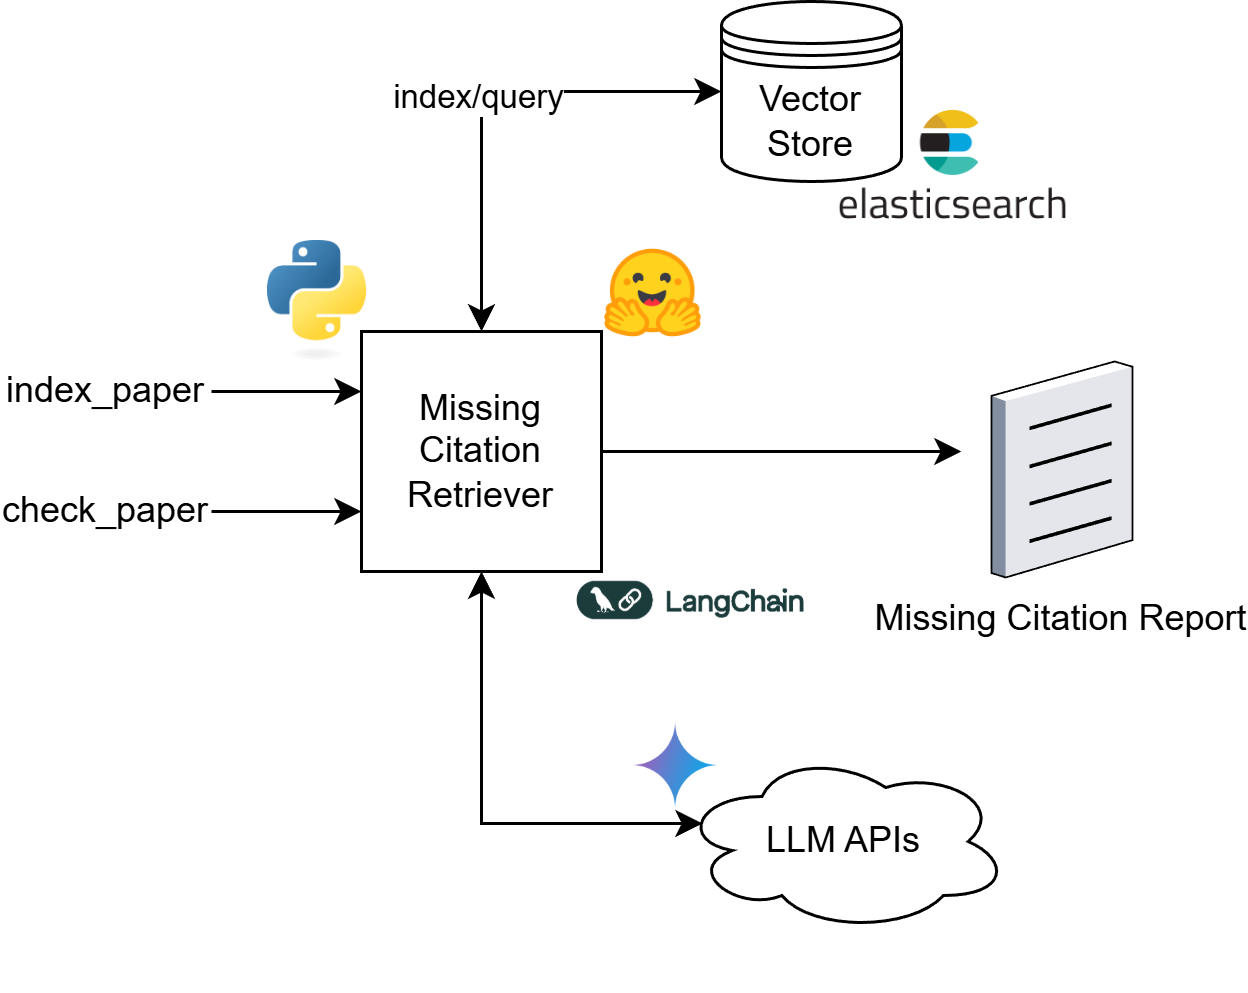
\includegraphics[width=\linewidth]{pics/software_diagram.png}
  \caption[Diagram describing the software architecture of our solution]{Visual representation of our solution's architecture}
  \label{fig:software-diagram}
\end{figure}

The culmination of all our experiments, the all-in-one pipeline described in \autoref{fig:citation-identification-diagram} and \autoref{fig:paper-pipeline}, is represented by two main entities:

\begin{itemize}
    \item a module called \textit{missing\_citation\_retriever} that exposes methods for indexing new papers in the database and running papers through the missing citation detection pipeline
    \item an external vector database that is used to store embeddings, accessed by the module when querying for candidates
\end{itemize}

A visual representation of this setup can be seen in \autoref{fig:software-diagram}. The module is written in Python, taking advantage of its vast ecosystem of high performance libraries for developing machine learning applications and ease of use. It handles processing papers that need to be indexed or verified for missing citations, communicates with the database when paper candidates are needed and handles LLM calls. The following sections will describe how we approached the implementation.

\section{Orchestration}

LLM app development is evolving at a break-neck pace with new models from different providers coming out constantly \cite{DeepSeekAI2024DeepSeekV3TR, Achiam2023GPT4TR, gemini-flash-2}. This makes it difficult to make correct design choices considering the fact that tomorrow's state-of-the-art model might be coming from a new company and have a radically different API. Therefore, due to our usage of large language models and text embeddings, we decided to organize our implementation using the LangChain framework\footnote{\url{https://python.langchain.com/}} for Python.

The purpose of the framework is to offer a fully featured solution for orchestrating LLM apps, providing interfaces to access different AI providers, databases, process documents etc. that are unified and easily interchangeable. This approach helps mitigate potential vendor lock-in and tech debt, allowing us to adapt as needed.

For instance, there is no need to translate between LLM APIs (Application Programmable Interfaces) if we decide to switch AI providers, all AI services are accessed through the same interface in LangChain. Similar features are present for vector databases and embedding models, allowing us to switch between them easily.

LangChain also helps organize workflows through its state graph feature, allowing us to model the different stages of our pipeline nodes which transmit information between them through their internal state. 

\section{Embeddings}

To generate embeddings of paper titles and abstracts, we use the HuggingFace transformers library \cite{Wolf2019HuggingFacesTS} directly through the unified LangChain interface. This allows us to easily access open-weight models such E5 Large Instruct \cite{Wang2024MultilingualET}.

Most paper abstracts are way too long to be encoded as a single embedding since the similarity score between our query and the entire abstract compared to the score between our query and smaller passages can be quite different. Even if this wasn't the case, most embedding models limit the number of tokens they accept as input due to performance issues, as the self-attention mechanism used by the transformer architecture scales \(O(n^2)\) to the length of the input in terms of memory and compute \cite{Pawar2024TheWW}. For instance, our model has a cap of 512 tokens, which almost certainly won't fit any abstracts.

This is why we need to split our text before generating embeddings. We concatenate the title and abstract for each paper that we want to index and split at 300 characters with an overlap of 100 characters between chunks to minimize the number of nonsensical passages. This provides a balance between the number of embeddings generated and the specificity of their content.

All embeddings are also normalized before being stored in the database, removing the magnitude/confidence of our vectors. This is the way our current model choice is recommended to be used and also serves as a small optimization that saves some compute at inference time since cosine similarity on normalized vectors is equivalent to dot-product, an operation that is easier to compute. A proof of this can be seen in \autoref{cosine_similarity}, it assumes that vectors A and B are already normalized, therefore their lengths are 1.

\begin{equation} \label{cosine_similarity}
cosine\_similarity(A, B) =  \frac{\mathbf{A} \cdot \mathbf{B}}{\|\mathbf{A}\| \, \|\mathbf{B}\|} = \frac{\mathbf{A} \cdot \mathbf{B}}{\mathbf{1} * \mathbf{1}} = dot\_product(A, B)
\end{equation}

\section{Vector Store}

We opted for Elasticsearch\footnote{https://www.elastic.co/enterprise-search} as a vector database because:
\begin{enumerate}
    \item it has a favorable open-source policy compared to a lot of proprietary solutions (Pinecone, Weaviate etc.).
    \item it allows storage of objects besides vectors, such as plain text and metadata, allowing us to use a single database instead of two.
    \item we can supplement our vector searches with filtering rules.
    \item it is way more flexible and easier to use than something like PostgreSQL + pgvector, being a NoSQL solution.
\end{enumerate}

Our database contains two indexes: one for plain text entries of papers and one for storing embeddings (and linking back to the plain text entries). This allows us to easily retrieve the title and abstract of a paper represented by a certain embedding without doing much computation during inference.

Of course, Elasticsearch can be easily replaced by any other vector database by altering a couple lines of code thanks to LangChain.

\section{LLM APIs}

Classifying sentences or re-ranking using API calls to large language models can be fairly slow, especially if we perform the calls sequentially by waiting for each individual call to finish before starting another one. To speed this process up, we employ concurrency through usage of a thread pool which waits for API calls to finish asynchronously, improving our IO-bound performance.

Chatbots, the classic LLM usage scenario, require some degree of randomness in their responses to avoid having deterministic outputs, allowing interaction with them to feel natural and less robotic. This randomness is provided by the temperature parameter, whose higher values offer the model a chance to select tokens besides the number one most likely next token. However, randomness is not at all beneficial to our classifier model since we want completely deterministic classifications. We will therefore set the temperature to 0 in our LLM calls.

Even though LangChain allows us to easily switch between AI providers for re-ranking if needed, the user might want to use different providers due to personal preference. The module offers the option to choose your provider through a strategy pattern, the current options being OpenAI and Gemini. This pattern also makes it easy to integrate other services in the future if desired.

\chapter{Evaluation} \label{evaluation}
% Acest capitol trebuie să răspundă, în principiu, la 2 întrebări și să se încheie cu o discuție a rezultatelor obținute. Cele doua întrebări la care trebuie sa se răspundă sunt:
% \begin{enumerate}
% 	\item  \textbf{Merge corect?} (Conform specificațiilor extrase în capitolul 2); 
% Evaluarea dacă merge corect se face pe baza cerințelor identificate în capitolele anterioare. 

% 	\item Cât de \textit{Bine} merge / cum se compară cu soluțiile existente? (pe baza unor metrici clare). 
% Evaluarea cât de \textit{Bine} merge trebuie să fie bazată pe procente, timpi, cantitate, numere, \textbf{comparativ cu soluțiile prezentate în capitolul 3}. Poate fi vorba de performanță, overhead, resurse consumate, scalabilitate etc. 
% \end{enumerate}

% În realizarea discuției, se vor utiliza tabele cu procente, rezultate numerice și grafice. În mod obișnuit, aici se fac comparații și teste comparative cu alte proiecte similare (dacă există) și se extrag puncte tari și puncte slabe. Se ține cont de avantajele menționate și se demonstrează viabilitatea abordării / aplicației, de dorit prin comparație cu alte abordări (dacă acest lucru este posibil). Cuvântul cheie la evaluare este ``metrică'': trebuie să aveți noțiuni măsurabile și cuantificabile. În cadrul procesului de evaluare, explicați datele, tabelele și graficele pe care le prezentați și insistați pe relevanța lor, în următorul stil: ``este de preferat ... deoarece …''; explicați cititorului nu doar datele ci și semnificația lor și cum sunt acestea interpretate. Din această interpretare trebuie să rezulte poziționarea proiectului vostru printre alternativele existente, precum și cum poate fi acesta îmbunătățit în continuare.

% Criterii pentru calificativul \textit{Bine}: 
% 
%        \cercetare Componentele și soluția în ansamblu au fost evaluate din punct de vedere al performanței, folosind seturi de date standard și cu o interpretare corectă a rezultatelor.
% 	     \ambele Discuție cu prezentarea calitativă și cantitativă a rezultatelor, precum și a relevanței acestor rezultate printr-o comparație complexă cu alte sisteme similare.

This chapter will provide a quantitative analysis of each step of our pipeline, comparing our solutions to the current state-of-the-art while discussing their respective advantages and drawbacks. To determine if our pipeline is a reasonable solution in terms of speed, we will evaluate its execution time across multiple input papers. Additionally, we will also discuss potential directions for future research based on these findings, highlighting ways in which our solution could be improved even further.

\section{Citing Sentence Detection} \label{evaluation-citsent}

As discussed in \autoref{gemini_citeworth}, the dataset we used for training and testing is CiteWorth \cite{Wright2021CiteWorthCD}. This is mostly due to it being the only dataset that attempts to improve the labeling process for this task through various heuristics, while also offering quantifiable metrics such as manual human evaluation compared to a baseline to determine its quality. All other comparable datasets \cite{Frber2018ToCO, Sugiyama2010IdentifyingCS} rely exclusively on automated labeling based on the presence of citation markers, a method which often leads to broken grammar and other features of low quality training examples.

Analyzing the accuracy and loss of the fine-tuned Gemini Flash 2.0 model during training, as seen in \autoref{fig:gemini2_train_metrics}\footnote{The metrics presented are based on next token prediction due to limitations of the external fine-tuning service we used.}, reveals that the model almost reaches its maximum performance on the validation set after a fairly low number of training steps (around 20), highlighting the power of transfer learning through fine-tuning large foundation models compared to classically training an architecture from scratch.

\begin{figure}[th]
\centering
\begin{subfigure}[t]{0.48\linewidth}
  \centering
  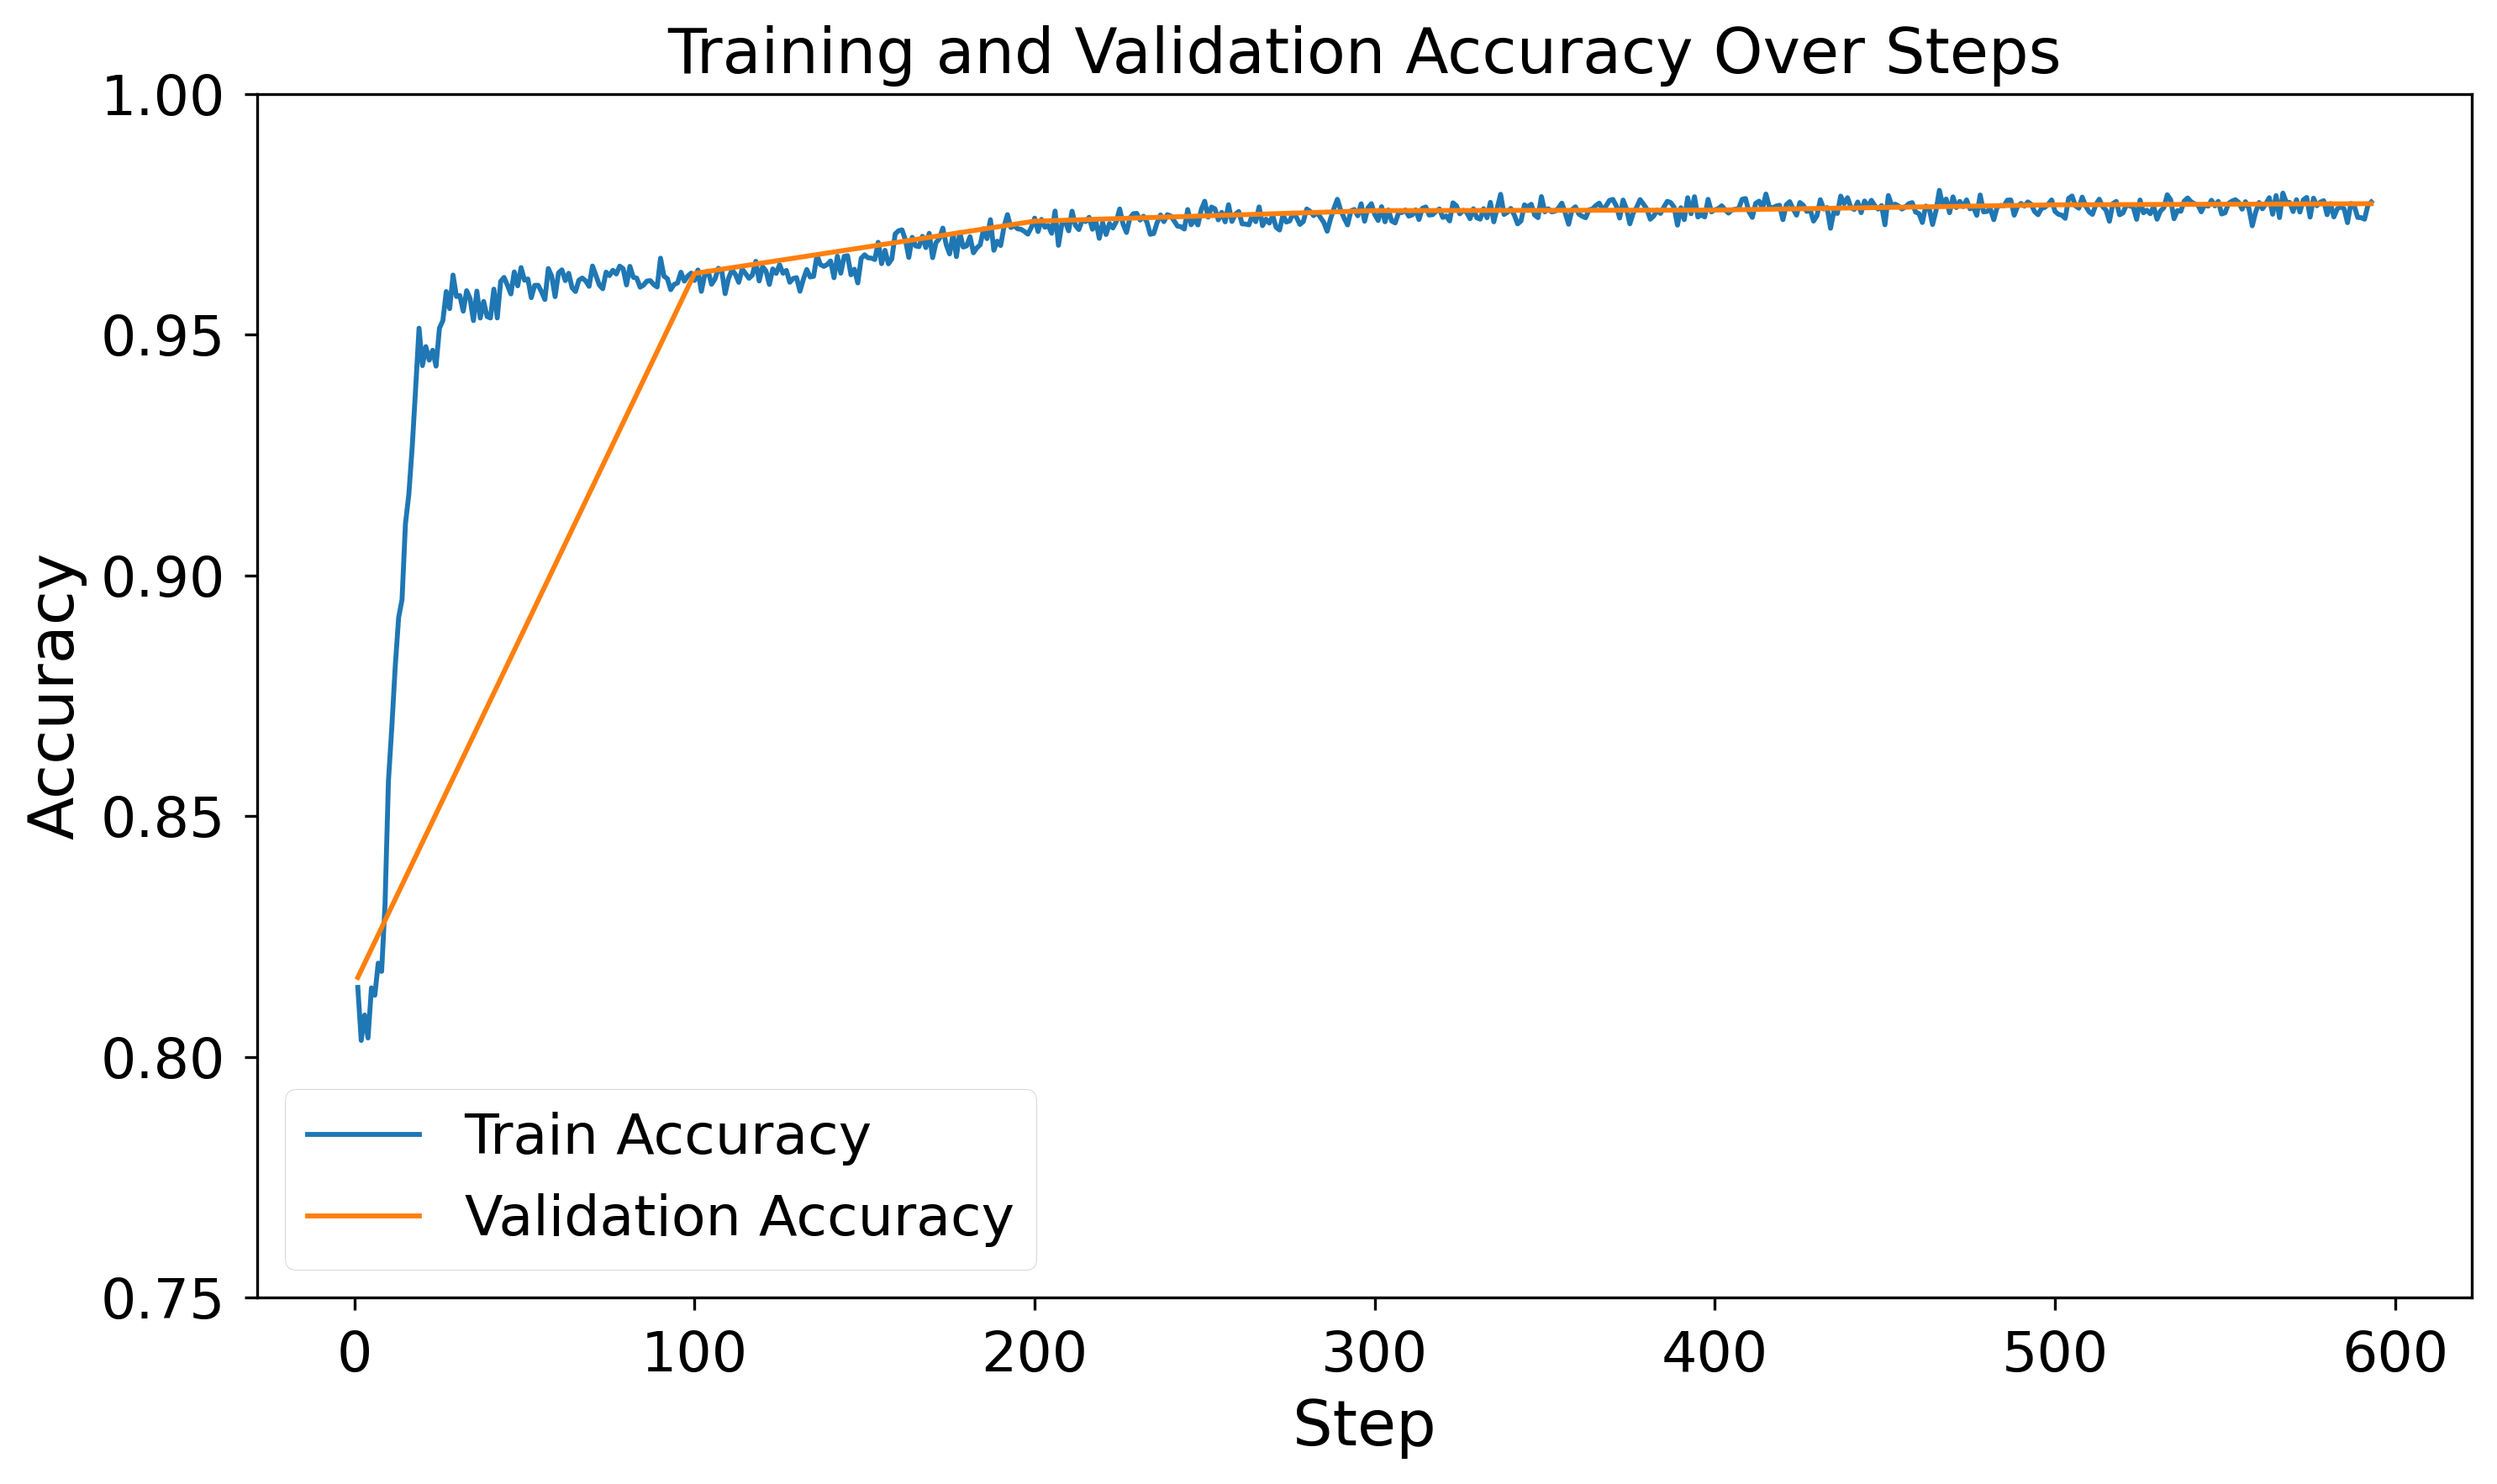
\includegraphics[width=\linewidth]{pics/gemini2_flash_training_validation_accuracy.png}
  \caption[Model accuracy between training steps on train and validation samples]{The model's accuracy between training steps on train and validation samples}
  \label{fig:gemini2_accuracy_train}
\end{subfigure}%
\hfill
\begin{subfigure}[t]{0.48\linewidth}
  \centering
  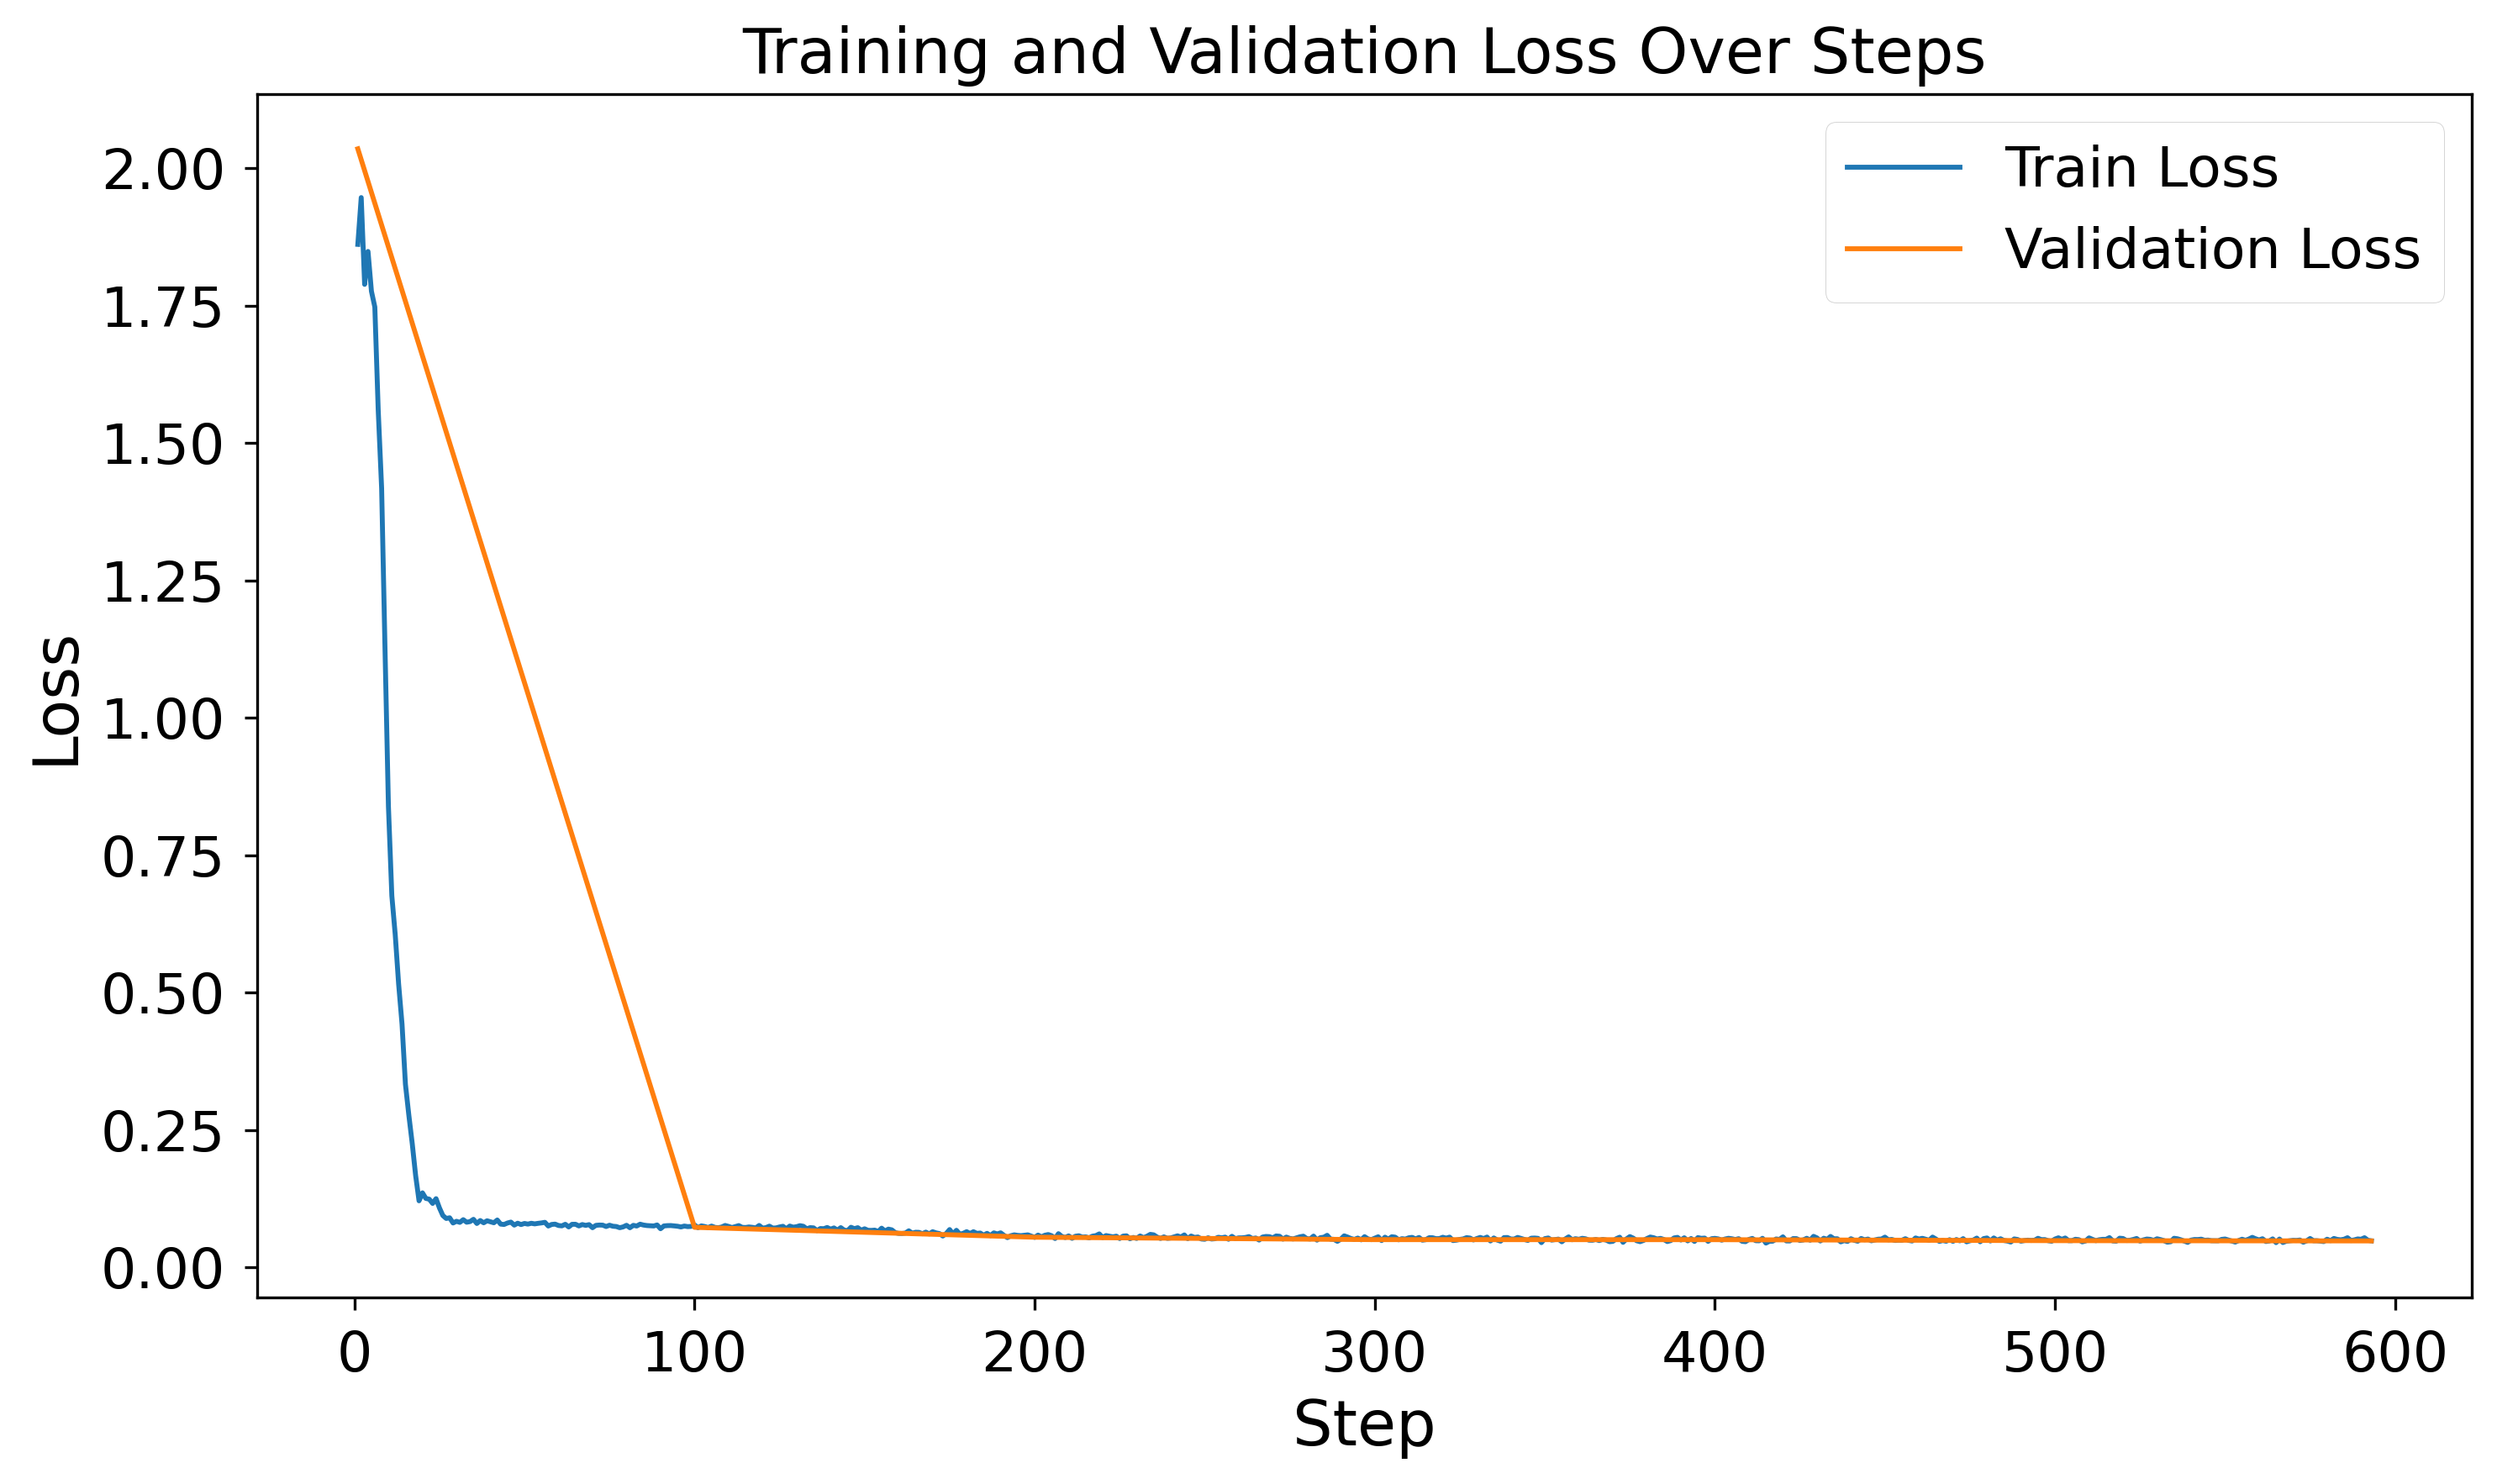
\includegraphics[width=\linewidth]{pics/gemini2_flash_training_validation_loss.png}
  \caption[Model loss between training steps on train and validation samples]{The model's loss between training steps on train and validation samples}
  \label{fig:gemini2_loss_train}
\end{subfigure}
\caption{Training and validation performance of the model over time.}
\label{fig:gemini2_train_metrics}
\end{figure}

Based on this observation, we can determine that the amount of data used for training was more than adequate since no significant gains were made after 200 steps of training. This means that we won't be able to improve on our solution by simply acquiring more data to train on. Therefore, if we want to get better performance from our model, further research should look toward other means of improvement. 

\begin{table}[th]
\centering
\small
\setlength{\tabcolsep}{16pt}
\renewcommand{\arraystretch}{1.2}
\begin{tabular}{lcccc}
\toprule
\textbf{Metric} & \textbf{Gemini Flash 2.0} & \textbf{Longformer} & \textbf{SciBERT} & \textbf{RCNN} \\
\midrule
Precision & \textbf{0.78} & 0.60 & 0.57 & 0.49 \\
Recall & 0.76 & \textbf{0.77} & 0.68 & 0.65 \\
F1-Score & \textbf{ 0.77} & 0.67 & 0.62 & 0.56 \\
\bottomrule
\end{tabular}
\caption{Evaluation of various citing sentence detection models on the test split of CiteWorth. SciBERT and RCNN performance was extracted from Wright et al. \cite{Wright2021CiteWorthCD}}
\label{tab:gemini-citsent-metrics}
\end{table}

\begin{figure}[th]
\centering
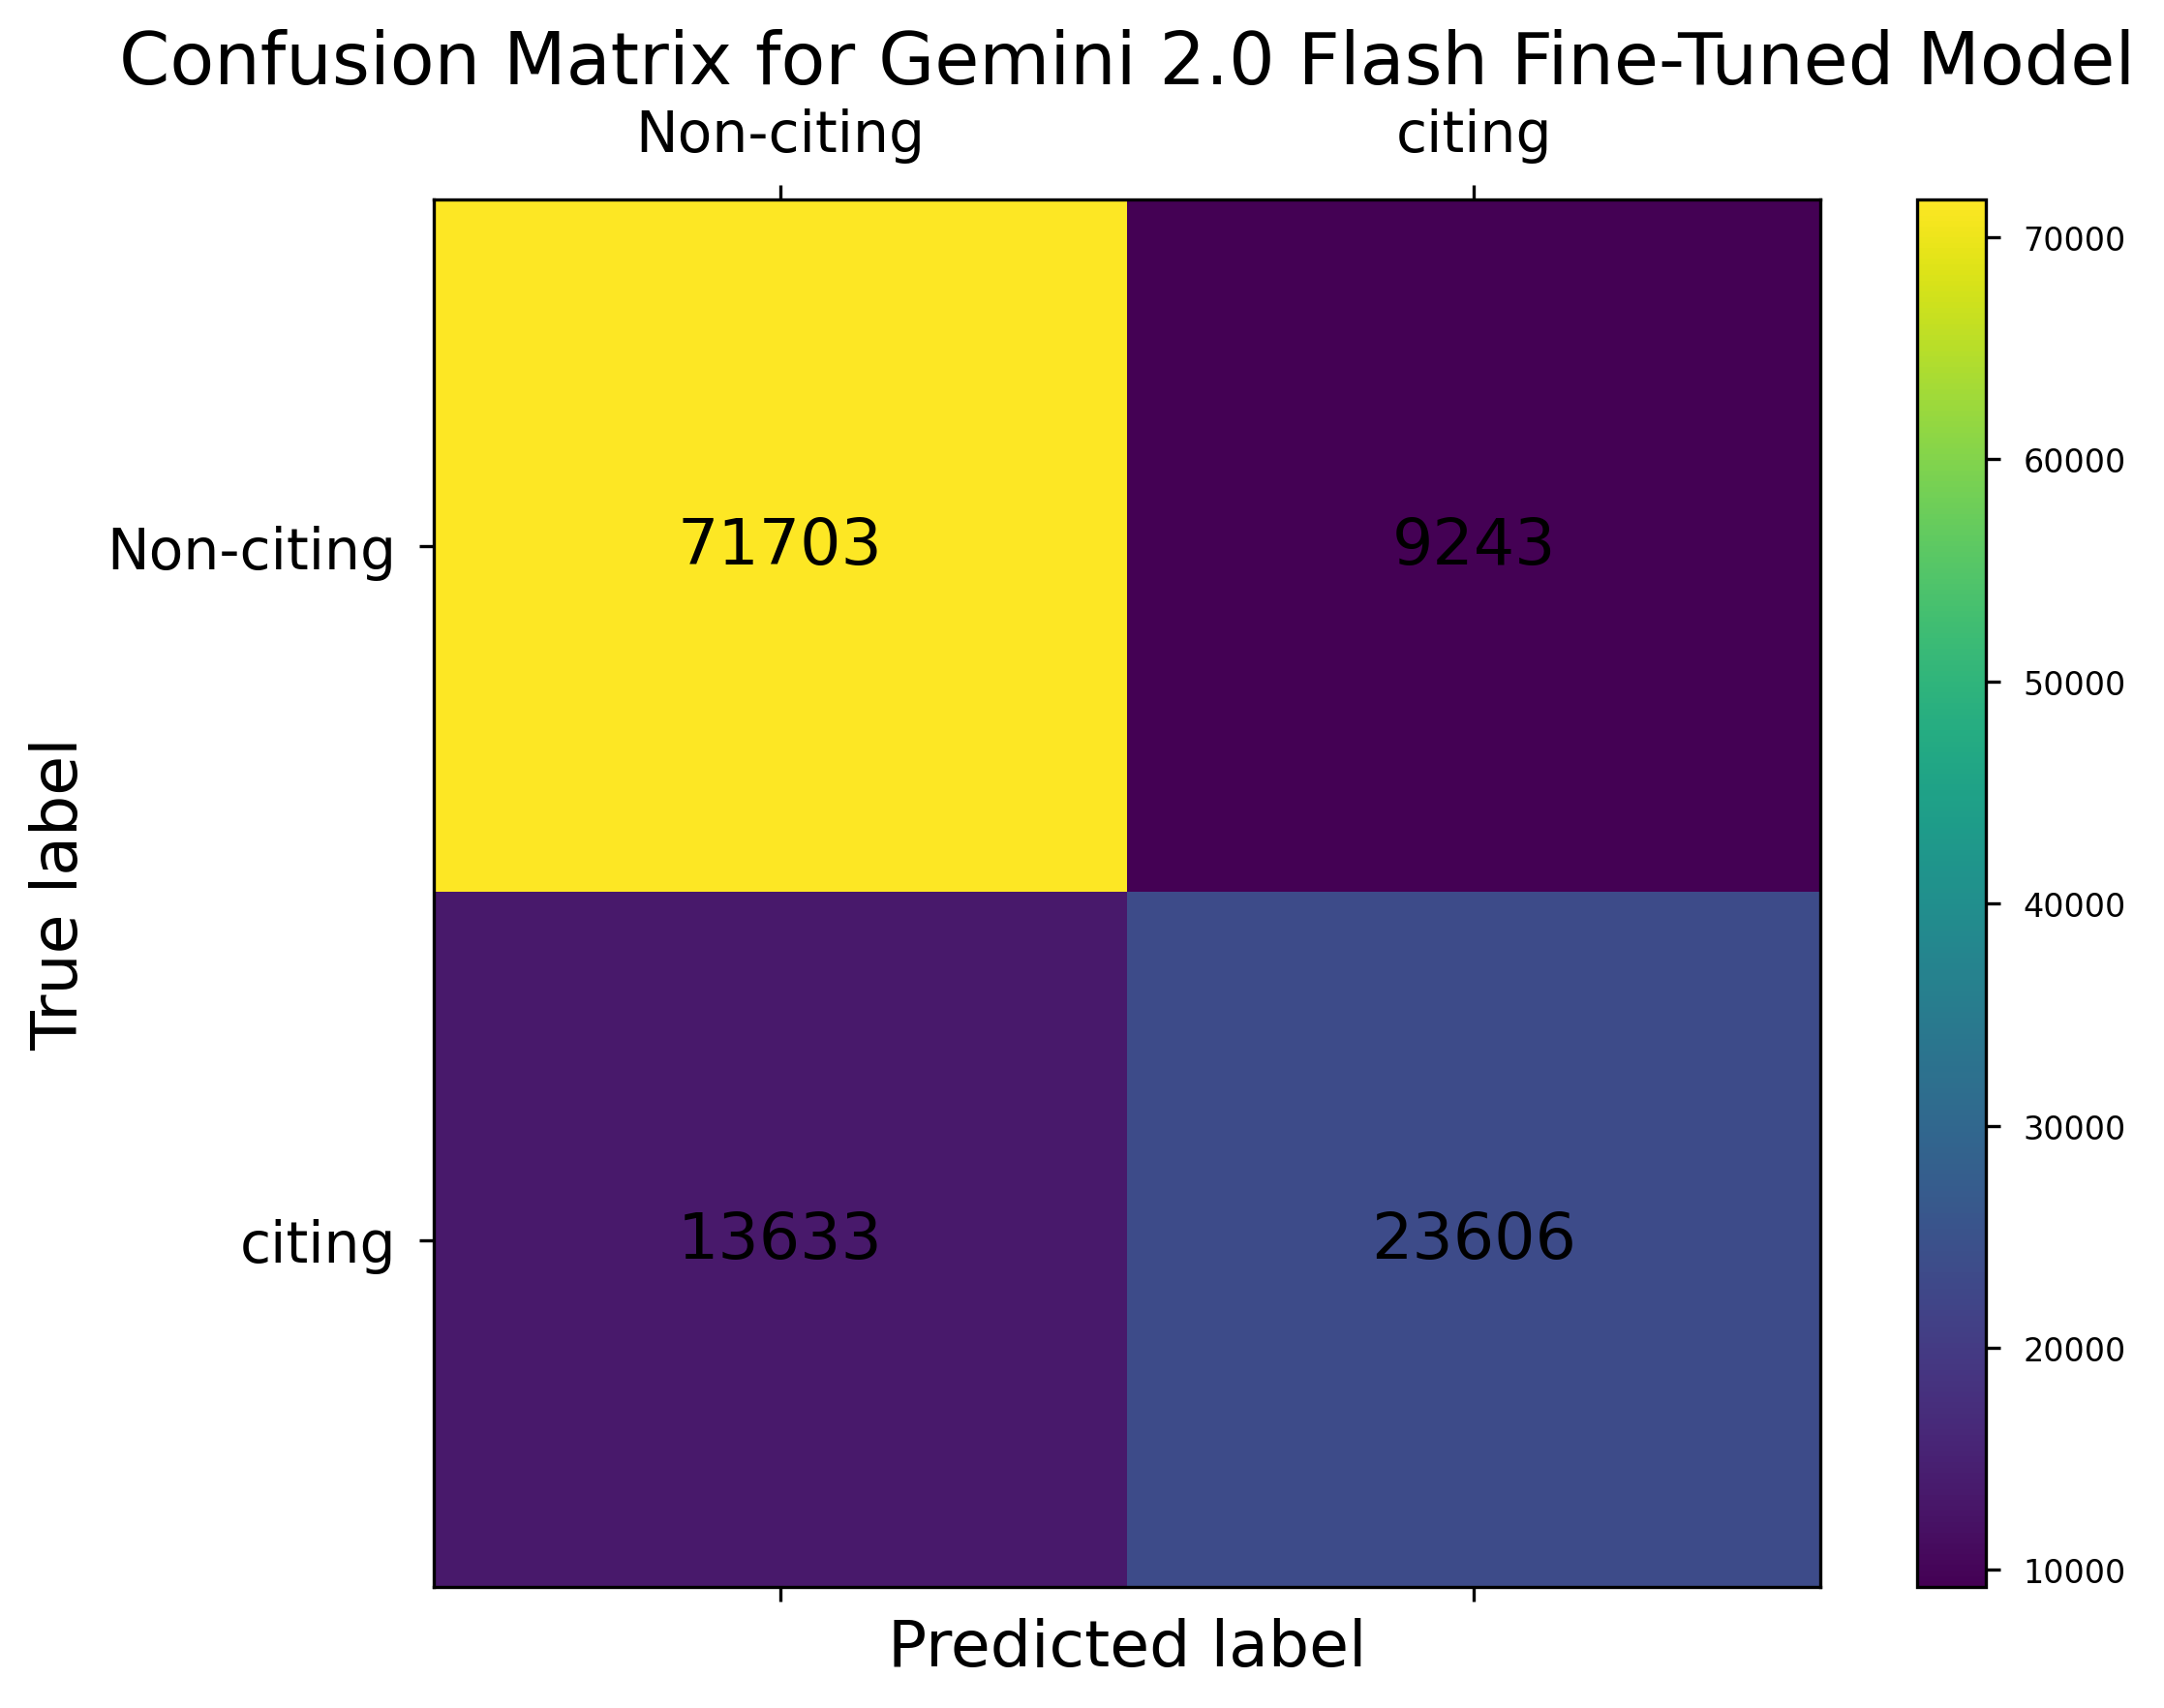
\includegraphics[width=14cm]{pics/gemini-citsent-confusion-matrix.png}
  \caption[Confusion matrix visualizing the predictions of our fine-tuned Gemini Flash 2.0 model on the test split of CiteWorth \cite{Wright2021CiteWorthCD}]{Visualization of the predictions of our fine-tuned Gemini Flash 2.0 model on the test split of CiteWorth \cite{Wright2021CiteWorthCD}}
  \label{fig:gemini-citsent-confusion-matrix}
\end{figure}

Using the test split of CiteWorth \cite{Wright2021CiteWorthCD} of over \(100k\) sentences, we performed a large scale evaluation of the fine-tuned model using accuracy, precision, recall and F1-Score as metrics \cite{M2015ARO}. The results of the evaluation can be analyzed in \autoref{tab:gemini-citsent-metrics} and more easily visualized through \autoref{fig:gemini-citsent-confusion-matrix}.

The most important metrics here are precision and recall (and implicitly F1-Score) due to a slight class imbalance of \(~60\%\) non-citing sentences to \(40\%\) citing sentences. Our model performs extremely well on these metrics, showing a 10 point F1-Score improvement over the next best model, Longformer. These findings prove our hypothesis that a full attention over a paragraph and a more complex model can highly improve performance on this task.

One of the drawbacks of our generative approach as opposed to other existing solutions is the possibility of outputs that do not respect the format used in the training data. For instance, there is nothing architecture-wise to force the model to provide labels for every single sentence in the input, meaning that it can very well decide to provide 3 labels for a 4 sentence paragraph. However, at least at our current scale, this does not seem to be a problem since the issue only popped up in one paragraph out of around \(21k\).

In our opinion, further research on this topic should approach the problem from a new perspective in terms of training input to achieve considerably better performance. A couple directions that could be explored:

\begin{itemize}
    \item expanding the attention mechanism to entire sections of papers as opposed to just paragraphs
    \item leveraging additional paper metadata (domain of study, journal etc.) as input
    \item exploiting the citation graph by taking already existing citations into account
\end{itemize}

Additionally, we think there is potential to match this performance with a less complex (and therefore local-friendly) large language model such as the 8 billion parameter model of the Llama 3 family \cite{Dubey2024TheL3} as our current approach might be overkill for the given task. Alternatively, our model can be swapped out for the Longformer if local inference and speed are desired over additional performance. 

\section{Retrieval} \label{sec:retrieval-eval}

We evaluated our citation candidate retriever on the PeerRead dataset \cite{Kang2018ADO}. This corpus features a set of papers that can be recommended and various passages (formally known as local citation contexts) which require citation recommendation. One advantage of this dataset is that it was sourced from peer reviews, a fairly realistic scenario for testing such a citation recommendation system. Details regarding this dataset can be observed in \autoref{tab:peerread-stats}.

\begin{table}[th]
\centering
\small
\setlength{\tabcolsep}{12pt}
\renewcommand{\arraystretch}{1.2}
\begin{tabular}{lccc}
\toprule
\textbf{Metric} & \textbf{Value} \\
\midrule
Paper count & 4,898 \\
Citation context count & 17,247 \\
Publication years & 2007 - 2017 \\
\bottomrule
\end{tabular}
\caption{Statistics regarding the PeerRead dataset \cite{Kang2018ADO}}
\label{tab:peerread-stats}
\end{table}

We measured our retriever's performance using the Recall@K metric, meaning how often the correct paper appears in the top K results. This allows us to evaluate the performance of our retrieval model for ranking relevant documents from fixed set of candidates.

We will compare our results to Jeong et al.'s \cite{Jeong2019ACC} and Yang et al.'s \cite{Yang2018ALB} neural network approaches on the same dataset to see how our method holds up to more potent, but less flexible models. These results can be observed in \autoref{tab:retriever-eval}.

Even though it may seem unfair to compare one step of our two-step recommendation system against unified solutions, it is important to keep in mind that we could have simply used one of these alternatives as retrievers. Therefore, it is important to compare the retriever as is, especially since it dictates the performance cap of the re-ranker. To exemplify this, if we want to re-rank the top 50 results, the performance of our re-ranker is currently capped at the value of Recall@50 for every single Recall@k value of the re-ranker. 

\begin{table}[th]
\centering
\small
\setlength{\tabcolsep}{12pt}
\renewcommand{\arraystretch}{1.2}
\begin{tabular}{lccccc}
\toprule
\textbf{Model} & \textbf{R@5} & \textbf{R@10} & \textbf{R@30} & \textbf{R@50} & \textbf{R@80} \\
\midrule
Yang et al. \cite{Yang2018ALB} & 0.21 & 0.27 & 0.41 & 0.48  & 0.55 \\
BERT-GCN \cite{Jeong2019ACC} & 0.48 & 0.52 & 0.60 & 0.65 & 0.69 \\
Our retriever & 0.20 & 0.27 & 0.37 & 0.46 & 0.51 \\
    \bottomrule
\end{tabular}
\caption{Retriever performance on the PeerRead dataset}
\label{tab:retriever-eval}
\end{table}

Though our approach is clearly outperformed by the BERT-GCN model of Jeong et al. \cite{Jeong2019ACC}, especially before re-ranking, the advantages of our model are worth the performance hit for our use case.

More specifically, the approaches used for comparison are very inflexible in terms of the set of papers they can recommend, meaning that they are limited to the papers they were trained on and modifications require retraining. Our retriever can adapt to new papers by just indexing some embeddings, offering excellent flexibility at the cost of some performance.

In terms of further research, it is clear that BERT-GCN \cite{Jeong2019ACC} dominates due to its exploitation of the larger citation graph. We think the next logical step is finding a way to incorporate this information into our retriever to improve results.

Another approach that could improve performance is fine-tuning our embedder to this specific task. This could be done by measuring its current performance against Recall@k metrics. However, there is a possibility that this would lead to similar issues of inflexibility as neural network approaches, meaning the model could learn to put queries close to the set of papers used for training in vector space, while external papers would be farther away.

The evaluation metrics used for this task could also be improved. Currently, two models that do not find the cited paper will score exactly the same, even if one of them has way more relevant recommendations compared to the other. Ideally, we'd have a way to compare sets of recommendations without needing the target paper to appear in them.

\section{Re-ranking}

To evaluate our re-ranker we used the top 50 candidate lists provided by retriever at the previous step and recalculated the Recall@k metrics after reordering, as seen in \autoref{tab:reranker-examples}.

Evaluating the re-ranker using this method makes its performance be highly influenced by the quality of the retriever since the target paper won't always be in the list of candidates. Because of this, we produce a second list of candidates by inserting the cited paper in it if it's not already present. This way, we can evaluate both the recommendation system as a whole, as well as the re-ranker independently.

\begin{table}[th]
\centering
\small
\setlength{\tabcolsep}{12pt}
\renewcommand{\arraystretch}{1.2}
\begin{tabular}{lcc}
\toprule
\textbf{Model} & \textbf{R@5} & \textbf{R@10} \\
\midrule
Yang et al. \cite{Yang2018ALB} & 0.21 & 0.27 \\
BERT-GCN \cite{Jeong2019ACC} & 0.48 & 0.52 \\
Our re-ranker (target paper always included) & 0.49 & 0.60 \\
Our re-ranker (candidates unmodified) & 0.28 & 0.32 \\
    \bottomrule
\end{tabular}
\caption{Re-ranker performance on the PeerRead dataset}
\label{tab:reranker-eval}
\end{table}

Unfortunately, these results mostly prove that our retriever is a bottleneck when it comes to matching the performance of other models, as our re-ranker is comparable to BERT-GCN \cite{Jeong2019ACC} in performance if the target paper is guaranteed to be present in the retriever. Of course, this scenario isn't realistic even with a better retriever, but the performance gap is large enough for us to justify this conclusion.

Despite this, our recommendation system still has a respectable performance and comes with some very valuable benefits, as described previously in \autoref{sec:retrieval-eval}, making it a better fit for expanding real world use cases which require high flexibility.

To improve re-ranking even further, we think different inputs should be explored as part of the reordering process to leverage the power of large language models to capture information through natural language. A couple of such inputs could be:

\begin{itemize}
    \item the powerful information encoded in the citation graph
    \item paper metadata (journal, domain etc.)
    \item additional text\footnote{Note: even though doing this would likely fill up the model's context window, our re-ranking method, RankGPT \cite{Sun2023IsCG,Sun2023InstructionDM}, has mechanisms to offset this.} from the paper (introduction, state-of-the-art section etc.)
\end{itemize}

This could allow the re-ranker to better understand the context in which the target paper situates in, allowing it to offer better recommendations at the cost of additional inference time due to larger inputs.

\section{Execution Time Analysis}

We ran our pipeline on 10 different scientific papers with page counts between 15 and 20 to estimate the time it takes to execute on a single input paper. Our experiment resulted in a mean average runtime of 39.5 seconds with a standard deviation of 17.44 seconds, meaning that our method's execution time is quite volatile. This is likely due to the fact that the number of passages which require citation recommendation varies from paper to paper.

While the execution time is not extraordinary, it is fast enough for integration in most applications. The only notable exceptions are real-time use cases such as text editors, a scenario in which 40 seconds whenever we want to identify missing citations is not acceptable as execution could be required after common actions such as edits.

As a workaround, such integrations could opt to only apply the pipeline on the paragraphs that suffered modifications since the previous verification. This would reduce the length of the target text, speeding up overall inference time.

\chapter{Conclusions}
% În acest capitol este sumarizat întreg proiectul, de la obiective, la implementare, si la relevanta rezultatelor obținute. În finalul capitolului poate exista o subsecțiune de ``Dezvoltări ulterioare''.

% Criterii pentru calificativul \textit{Bine}: 
% \begin{itemize}
% 	\item	Concluziile sunt corelate cu conținutul lucrării, și se oferă o imagine precisa asupra relevantei și calității rezultatelor obținute în cadrul proiectului. 
% \end{itemize}

In this paper, we introduced an end-to-end pipeline for finding missing citations in papers, leveraging the transformer architecture \cite{vaswani2023attentionneed}, instructional text embeddings for document retrieval, as well as large language models for re-ranking and classification.

The end result is an all-in-one solution that doesn't require any input besides the target paper to determine sentences with missing citations, as well as recommend fitting scientific works to cite in the detected contexts.

We also achieved state-of-the-art performance on the citing sentence detection task \cite{Sugiyama2010IdentifyingCS}, outperforming the current best solution, Wright et al.'s paragraph-level classifier \cite{Wright2021CiteWorthCD}, by 10 F1-score points.

The proposed recommendation system offers greater flexibility compared to alternative approaches, being capable of adapting to new sets of scientific papers that can be recommended by simply generating and indexing their embeddings in a database, no additional retraining needed. However, we did have to trade some performance for this benefit.

Our pipeline can easily be integrated into existing systems such as text editors or peer review platforms to mitigate the problem of missing citations in scientific publications, being fast enough for most use cases of scientific text analysis.

We think further improvements should exploit additional paper metadata, as well as the citation graph. These additions have the potential to improve both the citing sentence classifier and the recommendation, while keeping a similar degree of flexibility.

% \begin{itemize}
% 	\item 	NU utilizați referințe la Wikipedia sau alte surse fără autor asumat.
% 	\item 	Pentru referințe la articole relevante accesibile în web (descrise prin URL) se va nota la bibliografie și data accesării.
% 	\item 	Mai multe detalii despre citarea referințelor din internet se pot regăsi la:
% 	\begin{itemize}
% 		\item	\url{http://www.writinghelp-central.com/apa-citation-internet.html}
% 		\item	\url{http://www.webliminal.com/search/search-web13.html}
% 	\end{itemize}
% 	\item 	Note de subsol se utilizează dacă referiți un link mai puțin semnificativ o singură dată; Dacă nota este citată de mai multe ori, atunci utilizați o referință bibliografică.
% 	\item 	Dacă o imagine este introdusă în text și nu este realizată de către autorul lucrării, trebuie citată sursa ei (ca notă de subsol sau referință - este de preferat utilizarea unei note de subsol).
% 	\item 	Referințele se pun direct legate de text (de exemplu ``KVM [1] uses'', ``as stated by Popescu and Ionescu [12]'', etc.). Nu este recomandat să folosiți formulări de tipul ``[1] uses'', ``as stated in [12]'', ``as described in [11]'' etc..
% 	\item 	Afirmațiile de forma ``are numerous'', ``have grown exponentially'', ``are among the most used'', ``are an important topic'' trebuie să fie acoperite cu citări, date concrete si analize comparative.
% 	\begin{itemize}
% 		\item	Mai ales în capitolele de introducere, ``state of the art'', ``related work'' sau ``background'' trebuie să vă argumentați afirmațiile prin citări. Fiți autocritici și gândiți-vă dacă afirmațiile au nevoie de citări, chiar și cele pe care le considerați evidente.
% 		\item	Cea mai mare parte dintre citări vor fi în capitolele de introducere ``state of the art'', ``related work'' sau ``background''.
% 	\end{itemize}
% 	\item 	Toate intrările bibliografice trebuie citate în text. Nu le adăugați pur și simplu la final.
% 	\item 	Nu copiați sau traduceți niciodată din surse de informație de orice tip (online, offline, cărți, etc.). Dacă totuși doriți să oferiți, prin excepție, un citat celebru - de maxim 1 frază- utilizați ghilimele și evident menționați sursa. .
% 	\item 	Dacă reformulați idei sau creați un paragraf rezumat al unor idei folosind cuvintele voastre, precizați cu citare (referință bibliografică) sau cu notă de subsol sursa sau sursele de unde ați preluat ideile.
% \end{itemize}

% În Latex este foarte ușor să folosiți referințe într-un mod corect și unitar, fie prin adăugarea unei secțiuni
% \verb!\begin{thebibliography}!
% (vezi la sfârșitul acestei secțiuni), fie printr-un fișier separat de tip bib, folosind comanda
% \verb!\bibliography{}!,
% așa cum procedăm mai jos prin folosirea fișierului ``bibliography.bib''. În orice caz, în Latex va trebui să folosiți comanda
% \verb!\cite{}!
% pentru a adăuga referințe, iar această comandă trebuie folosită direct în text, acolo unde vreți sa apară citația, ca în exemplele următoare:

% \textbf{Important}: în această secțiune de obicei apar doar intrările bibliografice (adică doar listarea referințelor). Citarea lor prin comanda cite și explicații legate de ele trebuie facute în secțiunile anterioare. Citarea de mai sus a fost facută aici doar pentru exemplificare.

\newpage

% Asa se specifica folosirea unui fisier cu referinte bibliografice:
\bibliographystyle{unsrt} % alternative is plain
\addcontentsline{toc}{chapter}{Bibliography}  
\bibliography{bibliography}

\end{document}
